% 6-8 pages.
% Due May 31, 2016.

\documentclass[11pt]{article}

\usepackage[T1]{fontenc}
\usepackage{lmodern}
\usepackage{hyperref}
\usepackage[ruled, linesnumbered]{algorithm2e}
\usepackage{bm}
\usepackage{epsf,graphicx,amssymb,amsmath,amsbsy,authblk}
\usepackage[english]{babel}
\usepackage{psfrag}
\usepackage{fancyhdr}
\usepackage{mathrsfs}
\usepackage{natbib}
\usepackage{xcolor}
\usepackage{multirow} % added by Pasche

% Algebraic rings.
\newcommand*{\Complex}{\mathbb{C}}
\newcommand*{\Binary}{\mathbb{F}_2}
\newcommand*{\Ints}{\mathbb{Z}}
\newcommand*{\Reals}{\mathbb{R}}

% Operators.
\renewcommand*{\L}{\mathscr{L}}
\renewcommand*{\O}{\mathcal{O}}
\renewcommand*{\d}[3][1]{%
    \if#11
    \frac{d #2}{d #3}
    \else
    \frac{d^#1 #2}{d #3^#1}
    \fi%
}
\newcommand*{\half}{^{1/2}}
\newcommand*{\invhalf}{^{-1/2}}
\newcommand*{\ip}[2]{\left<#1, #2\right>}
\newcommand*{\p}[3][1]{%
    \if#11
    \frac{\partial #2}{\partial #3}
    \else
    \frac{\partial^#1 #2}{\partial #3^#1}
    \fi%
}

% Matrices.
\newcommand*{\A}{\mathbf{A}}
\renewcommand*{\H}{\mathbf{H}}
\newcommand*{\I}{\mathbf{I}}
\renewcommand*{\P}{\mathbf{P}}
\newcommand*{\X}{\mathbf{X}}
\newcommand*{\W}{\mathbf{W}}
\newcommand*{\PHI}{\mathbf{\Phi}}
\newcommand*{\PSI}{\mathbf{\Psi}}
\newcommand*{\SIGMA}{\mathbf{\Sigma}}

% Vectors.
\renewcommand*{\a}{\mathbf{a}}
\renewcommand*{\c}{\mathbf{c}}
\newcommand*{\f}{\mathbf{f}}
\newcommand*{\ft}{\tilde{\f}}
\renewcommand*{\r}{\mathbf{r}}
\newcommand*{\w}{\mathbf{w}}
\newcommand*{\x}{\mathbf{x}}
\newcommand*{\z}{\mathbf{z}}
\newcommand*{\epsilonv}{\bm{\epsilon}}
\newcommand*{\phiv}{\bm{\phi}}
\newcommand*{\psiv}{\bm{\psi}}
\newcommand*{\zero}{\mathbf{0}}

% hyperref commands.
\renewcommand*{\sectionautorefname}{Section}
\renewcommand*{\subsectionautorefname}{\sectionautorefname}

% Other commands.
\newcommand{\KSE}{Kuramoto--Sivashinsky equation}
\newcommand{\kkc}[1]{\textcolor{red}{[KKC: #1]}}
\newcommand{\eec}[1]{\textcolor{red}{[EEC: #1]}}

\marginparwidth 0pt
\oddsidemargin 0pt
\evensidemargin 0pt
\marginparsep 0pt
\topmargin -50pt
\textwidth 17cm
\textheight 22.0cm
\headheight 13.6pt
\pagestyle{fancy}

\lhead{{\it Montestigliano Workshop}}
\rhead{{\it 2016 Reports}}

% Bibliography styles.
\bibliographystyle{plainnat}
\setcitestyle{}

\graphicspath{{figures/}}

\begin{document}

\begin{center}
    {\bf \Large Modeling the Kuramoto--Sivashinsky Equation}\\
    \vspace{0.3cm}
    {%
        \large{%
            Victor Beltran,\footnote{Universidad Polit\'ecnica de Madrid}
            Kevin K. Chen,\footnote{University of Southern California}
            Emma Cooke,\footnote{Imperial College London} and
            Simon Pasche\footnote{\'Ecole Polytechnique F\'ed\'erale de Lausanne}%
        }%
    }
\end{center}
\vspace{0.3cm}

\begin{abstract}
    We investigate the nonlinear dynamics and modeling of the \KSE.
    Both the parallel equation with periodic boundary conditions, as well as a non-parallel equation on an infinite domain, are considered.
    In both equations, we report three cases where the stable solution is the trivial solution, a simple periodic orbit of a single frequency, and a more complex periodic orbit exhibiting multiple harmonics.
    In particular, the parallel periodic equation has analytical eigenvalues and eigenmodes, which allow an simple characterization of the Hopf bifurcation.
    The various types of solutions are demonstrated with phase portraits.
    Next, we compute POD-DEIM modes and reduced-order models for the parallel equation.
    Not only does POD-DEIM capture the limit cycle with a comparatively small number of modes, but also, transient modes correctly capture the limit cycle, and limit cycle modes correctly capture the transients.
\end{abstract}

\section{Introduction}

The \KSE\ is a fourth-order partial differential equation in time and one-dimensional space that arises in many physical phenomena.
The equation was independently discovered by \cite{KuramotoPTP76} in the context of wave propagation in reaction--diffusion systems, and \cite{SivashinskyAA77} in the context of laminar flames.
Since then, the equation has also been derived for thin film flows, interfacial instabilities, drift waves in plasmas \citep[see][]{KevrekidisSIAMJAM90}, Tollmien--Schlichting waves in flat-plate boundary layers \citep{FabbianeAMR14}, and many more applications.

One of the features that makes the \KSE\ a common model problem is the complex hierarchy of attractors for different equation parameters.
The range of stable solutions, as discussed by \cite{KevrekidisSIAMJAM90}, includes fixed points, simple periodic orbits, more complex periodic orbits (e.g., exhibiting multiple frequencies), quasi-periodic orbits, and ultimately chaos.
Therefore, many have characterized the equation's complex dynamics using simple reduced-order models, often taking advantage of symmetry \citep[e.g.,][]{AubrySIAMJSC93, RowleyPD00}.

Proper orthogonal decomposition---also known as principal component analysis and Karhunen--Lo\`eve expansion---is a very common data-based modal decomposition, and is discussed in works by \cite{SirovichQAM87} and \cite{HolmesTCSDSS}.
Given a set of data snapshots, the technique extracts orthogonal modes that optimally capture the energy of the input data.
These modes are then typically used in Galerkin models to form reduced order models.
Despite the popularity of POD-based reduced order models, the technique suffers from a number of shortcomings.
In particular, the construction of nonlinear terms in POD models may be computationally expensive.

The discrete empirical interpolation method \citep[DEIM;][]{ChaturantabutIEEECDC09, ChaturantabutRice09a} addresses the last concern by intelligently selecting discrete points in the domain for which the nonlinear term is computed, and neglecting all other points.
Although other nonlinear POD models exist \citep[see, e.g.,][]{NoackJFM03}, the DEIM method has been shown to be very computationally efficient and to create very accurate POD models.
Although error bounds have been derived for DEIM, the precise reasons for its success have not been rigorously proven.

In this report, we cover two topics related to the \KSE.
First, we use linear stability theory and computation to characterize the equation's simple attractors.
Second, we demonstrate the success of POD-DEIM reduced-order models for this equation.
The \KSE\ and POD-DEIM are first reviewed in \autoref{sec:theory}, and our numerical methods in~\autoref{sec:methods}.
Next, the attractors are described in \autoref{sec:attractors}, and the application of POD-DEIM is demonstrated in \autoref{sec:pod-deim}.
Finally, we summarize our work in \autoref{sec:conclusions}.

\section{Theory}
\label{sec:theory}

\subsection{The \KSE}
\label{sec:ks}

In this report, we cover two different forms of the \KSE.
Given the streamwise displacement $x$ and time $t$, the dependent variable $w(x, t) : \Reals \times \Reals \to \Reals$ obeys the nonlinear equation
\begin{equation}
    \label{eq:ks}
    \p{w}{t} = \L w - w \p{w}{x},
\end{equation}
where the linear operator $\L$ is given by
\begin{equation}
    \label{eq:ks-linear}
    \L := - \left(U \p{}{x} + \p{}{x} \left(\mu_0 \p{}{x}\right) + \gamma \p[4]{}{x}\right).
\end{equation}

In the parallel form, we assume a periodic domain $x \in [-1, 1]$.
We also define positive real constants $U, \mu_0, \gamma$ respectively corresponding to the advection velocity, anti-diffusion, and short-wavelength diffusion.
The role of each term can be seen by examining a snapshot in time of the form $w = e^{i \pi n x}$ for wavenumbers $n \in \Ints$.
The two first derivative terms correspond to advection at the speed $U + w$, as in the Burgers' and Navier--Stokes equation;
the second derivative term evaluates to $(\pi n)^2 \mu_0 w$ and is therefore antidiffusive and destabilizing;
and the fourth derivative term evaluates to $- (\pi n)^4 \gamma w$ and is therefore diffusive and stabilizing, especially at short wavelengths.
The non-parallel form of the \KSE\ that we will consider is the same, except that we employ $\mu_0(x) = e^{-x^2}$ and consider the infinite domain $x \in \Reals$, where assume that $w$ is well-behaved at $x \to \pm \infty$.

For both forms, we remark that the $U \, \partial / \partial x$ term is actually optional---$w$ could be replaced with $U + w$ and the $U \, \partial / \partial x$ term removed, and the equations will remain the same.
In fact, most works omit the $U \, \partial / \partial x$ term in their analyses.
The purpose of this term is to allow the base flow to be fixed at $w(x, t) = 0$, which corresponds to an advection speed of any arbitrary $U$.

\subsection{POD-DEIM}

Proper orthogonal decomposition \citep{SirovichQAM87, HolmesTCSDSS} is a method of identifying dominant directions in a size $m$ set of data $\{\x_k\}_{k=1}^m$, with $\x_k \in \Complex^n$ for $k = 1, \ldots, m$.
(It is common in many problems to restrict $\x_k$ to $\Reals^n$.)
The modes are ranked in a particular order so that the first $r$ modes maximize the orthogonal projection of the data onto the span of those modes for each $r = 1, \ldots, m$.
Given an inner product $\ip{\cdot}{\cdot} : \Complex^n \times \Complex^n \to \Complex$ and the Kronecker delta $\delta_{jk}$, we therefore write the POD modes as the set of vectors $\phiv_j \in \Complex^n$ for $j = 1, \ldots, m$ such that
\begin{subequations}
    \begin{align}
        \sum_{k=1}^m \left\|\x_k - \sum_{j=1}^r \ip{\x_k}{\phiv_j} \phiv_j \right\|_2^2 \quad & \text{is minimized for each } r = 1, \ldots, m, \\
        \ip{\phiv_j}{\phiv_k} = \delta_{jk}.
    \end{align}
\end{subequations}
In reduced-order modeling, it is common to truncate the POD mode set and only consider the proper subset $\{\phiv_j\}_{j=1}^r$ for $1 \le r \ll m$, with the assumption that most interesting features of $\{\x_k\}_{k=1}^m$ are contained in only $r$ modes.

The computation of POD is straightforward.
Let us assume the common case where $m \le n$, and let $(\cdot)^*$ indicate the conjugate transpose.
Also, consider the inner product $\ip{\cdot}{\cdot} : \Complex^n \times \Complex^n \to \Complex; \z_j, \z_k \mapsto \z_k^* \H \z_j$, where typically, $\H \in \Reals^{n \times n}$ is a diagonal matrix with the positive grid sizes on the diagonal.
(On uniform grids, we would normally have $\H = \I$.)
Given the data matrix $\X := \begin{bmatrix} \x_1 & \ldots & \x_m \end{bmatrix} \in \Complex^{n \times m}$, the economy-sized singular value decomposition (SVD) of $\H\half \X$ is
\begin{equation}
    \label{eq:svd}
    \H\half \X = (\H\half\PHI) \SIGMA \W^*,
\end{equation}
where $\PHI \in \Complex^{n \times m}$ and $\PHI^* \H \PHI = \I$, $\SIGMA \in \Reals^{m \times m}$ is a diagonal matrix with $\{\sigma_k\}_{k=1}^m$ on the diagonal such that $\sigma_1 \ge \cdots \ge \sigma_m \ge 0$, and $\W \in \Complex^{m \times m}$ and $\W^* \W = \W \W^* = \I$.
The POD modes are then the columns of $\PHI = \begin{bmatrix} \phiv_1 & \cdots & \phiv_m \end{bmatrix}$.
From this point forward, we will truncate and redefine the POD matrix by $\PHI := \begin{bmatrix} \phiv_1 & \cdots & \phiv_r \end{bmatrix} \in \Complex^{n \times r}$.

The primary challenge in nonlinear modeling is to capture nonlinear dynamics in a way that is both accurate and computationally efficient.
The POD-DEIM algorithm \citep{ChaturantabutIEEECDC09, ChaturantabutRice09a} addresses this issue as follows.
Suppose that the discrete-space dynamics contain the nonlinear function $\f : \Complex^n \to \Complex^n$, and the dynamics are given for $\x(t) \in \Complex^n$ by
\begin{equation}
    \d{\x}{t} = \A \x + \f(\x).
\end{equation}
We restrict $\x$ to the span of $\{\phiv_j\}_{j=1}^r$ by assigning POD mode coefficients $\a(t) := \begin{bmatrix} a_1(t) & \cdots & a_r(t) \end{bmatrix} \in \Complex^r$ such that $\x(t) = \PHI \a(t)$.
Using this projection, we arrive at
\begin{equation}
    \label{eq:galerkin}
    \d{\a}{t} = \PHI^* \H \A \PHI \a + \PHI^* \H \f(\PHI \a),
\end{equation}
but the nonlinear term must still be computed over $\Complex^n$.

Therefore, we also compute POD modes $\psiv_j \in \Complex^n$ for $j = 1, \ldots, s$ from the nonlinear terms $\f(\x_1), \ldots, \f(\x_m)$, and we define $\PSI := \begin{bmatrix} \psiv_1 & \cdots & \psiv_s \end{bmatrix}$.
Next, we project the output of $\f$ to the span of $\{\psiv_j\}_{j=1}^s$, such that for some coefficient vector $\c \in \Complex^s$, error vector $\epsilonv \in \Complex^n$, and input $\x \in \Complex^n$,
\begin{equation}
    \f(\x) = \PSI \c + \epsilonv
\end{equation}
and $\ip{\epsilonv}{\psiv_j} = 0$ for $j = 1, \ldots, s$.
To reduce the computation of $\f$ to one over $\Complex^s$, we use the DEIM algorithm (Algorithm~\ref{algo:deim})%
\begin{algorithm}[t]
    \caption{
        Discrete empirical interpolation method;
        $\PSI_j$ and $\P_j$ respectively denote the matrices comprised of first $j$ columns of $\PSI$ and $\P$, and $P_{j, k}$ denotes the entry of $\P$ in row $j$ and column $k$.%
    }
    \label{algo:deim}

    \DontPrintSemicolon
    \SetAlgoLined

    \KwData{Nonlinear POD modes $\PSI := \begin{bmatrix} \psiv_1 & \cdots & \psiv_s \end{bmatrix} \in \Complex^{n \times s}$}
    \KwResult{DEIM projection matrix $\P \in \Binary^{n \times s}$}

    $m \leftarrow \arg \max |\psiv_1|$ \;
    $\P \leftarrow 0^{n \times s}$ \;
    $P_{m, 1} \leftarrow 1$ \;
    \For{$j = 2, \ldots, s$} {
        $\r \leftarrow (\I - \PSI_{j-1} (\P_{j-1}^* \PSI_{j-1})^{-1} \P_{j-1}^*) \psiv_j$ \;
        $m \leftarrow \arg \max |\r|$ \;
        $P_{m, j} \leftarrow 1$ \;
    }
\end{algorithm}
to choose a projection matrix $\P \in \Binary^{n \times s}$ that consists of all zeros, except that each column has one unique index for which the entry is one.
Thus, $\P^* \f(\x) = \P^* \PSI \c + \P^* \epsilonv$; if $\P^* \PSI$ is full-rank, then $\c = (\P^* \PSI)^{-1} \P^* (\f(\x) - \epsilonv)$, and hence,
\begin{equation}
    \label{eq:nonlinear-projection}
    \f(\x) = \PSI (\P^* \PSI)^{-1} \P^* \f(\x) + (\I - \PSI (\P^* \PSI)^{-1} \P^*) \epsilonv.
\end{equation}

To complete the POD-DEIM procedure, we make two assumptions: first, we assume that
\begin{equation}
    \label{eq:zero-error}
    (\I - \PSI (\P^* \PSI)^{-1} \P^*) \epsilonv = \zero
\end{equation}
(i.e., the nonlinear POD modes perfectly capture the nonlinear dynamics), and second, we assume that there exists a pointwise version $\ft : \Complex^s \to \Complex^s$ of $\f$ such that
\begin{equation}
    \label{eq:pointwise}
    \P^* \f(\x) = \ft(\P^* \x).
\end{equation}
That is, $\P^* \f(\x)$ first computes $\f(\x)$ and then selects discrete elements of the output to keep; on the other hand, $\ft(\P^* \x)$ first selects discrete elements of the \emph{input}, and computes the nonlinearity only on those elements.
We remark that this shortcut is generally allowed, even if $\f$ does not appear to be a pointwise operation, e.g., if it involves spatial derivatives.
For instance, suppose that $\f(\x)$ is the discrete-space formulation of the function $f(w) = -w \, \partial w / \partial x$, as in~\eqref{eq:ks}.
To evaluate $\ft(\P^* \x)$, one would simply evaluate both $-w$ and $\partial w / \partial x$ at the DEIM points $x_j$ corresponding to the nonzero elements of the columns of $\P$, and multiply the result.

Finally, we combine (\ref{eq:galerkin}, \ref{eq:nonlinear-projection}--\ref{eq:pointwise}) to obtain the reduced-order model
\begin{equation}
    \d{\a}{t} = \PHI^* \H \A \PHI \a + \PHI^* \H \PSI (\P^* \PSI)^{-1} \ft(\P^* \PHI \a).
\end{equation}
The matrices $\PHI^* \H \PSI (\P^* \PSI)^{-1} \in \Complex^{r \times s}$ and $\P^* \PHI \in \Complex^{s \times r}$ should be pre-computed for maximal efficiency.
We remark that it is never actually necessary to represent or use $\P^*$ explicitly in computations; in software, it is sufficient just to use its nonzero entries to manipulate the indices of its operand.
In addition, we will employ $s = r$ for simplicity in this report.

\section{Numerical methods}
\label{sec:methods}

In the parallel \KSE, we use the Fourier pseudospectral method described by \cite{WeidemanACMTMS00} to compute differentiation matrices.
To reduce minimize the amplification of short-wavelength noise by the fourth derivative, we employ the 36th order filter described by \cite{HouJCP07} for the diffusion term.
We use the uniform spatial discretization $\Delta x = 0.005$, such that the periodic domain $x \in [-1, 1]$ is comprised of 400 grid points.
The parallel equation is simulated and analyzed in MATLAB.

In the non-parallel \KSE, we use the finite element software FreeFem++ \citep{HechtJNM12}, employing 4,000 equispaced elements with width $\Delta x = 0.05$ on the domain $x \in [-100, 100]$.
Homogeneous Dirichlet conditions are set at $x = -100$, and outflow conditions are set at $x = 100$.
The shift-and-invert variant of the Arnoldi method \citep[see][]{TrefethenNLA} is used to compute the leading eigenvalues and eigenmodes of the linearized dynamics.

\section{Characterizations of attractors}
\label{sec:attractors}

\subsection{Parallel equation}

In the parallel equation, the eigendecomposition of the linear dynamics $\L$ about the base flow $w(x) = 0$ can be expressed analytically.
Because of the domain periodicity, we assume eigenmodes of the form $w_n(x) = e^{i \pi n x}$ for $n \in \Ints$.
The eigendecomposition $\L w_n = \lambda_n w_n$, for $\lambda_n \in \Complex$, therefore yields $\lambda_n = (\pi n)^2 (\mu_0 - (\pi n)^2 \gamma) - i \pi n U$.
Then $n = 0$ eigenmode---corresponding to $\lambda_0 = 0$---is simply the mode where $w(x)$ is a constant, and is related to the arbitrary velocity scale discussed in \autoref{sec:ks}.
Besides this mode, all other eigenmodes have a nonzero imaginary part.
Examining the structure of the real part of $\lambda_n$, it is evident that the $n = \pm 1$ mode is the least stable mode.
In particular, the $n = \pm 1$ mode undergoes a Hopf bifurcation when $\gamma = \mu_0 / \pi^2$.
The corresponding eigenvalue reveals that the base flow is stable when $\gamma > \mu / \pi^2$ and unstable when $\gamma < \mu / \pi^2$.

\kkc{Fill in the rest.}

\autoref{fig:time-resolved}(a) depicts\ldots

\begin{figure}
    \centering
    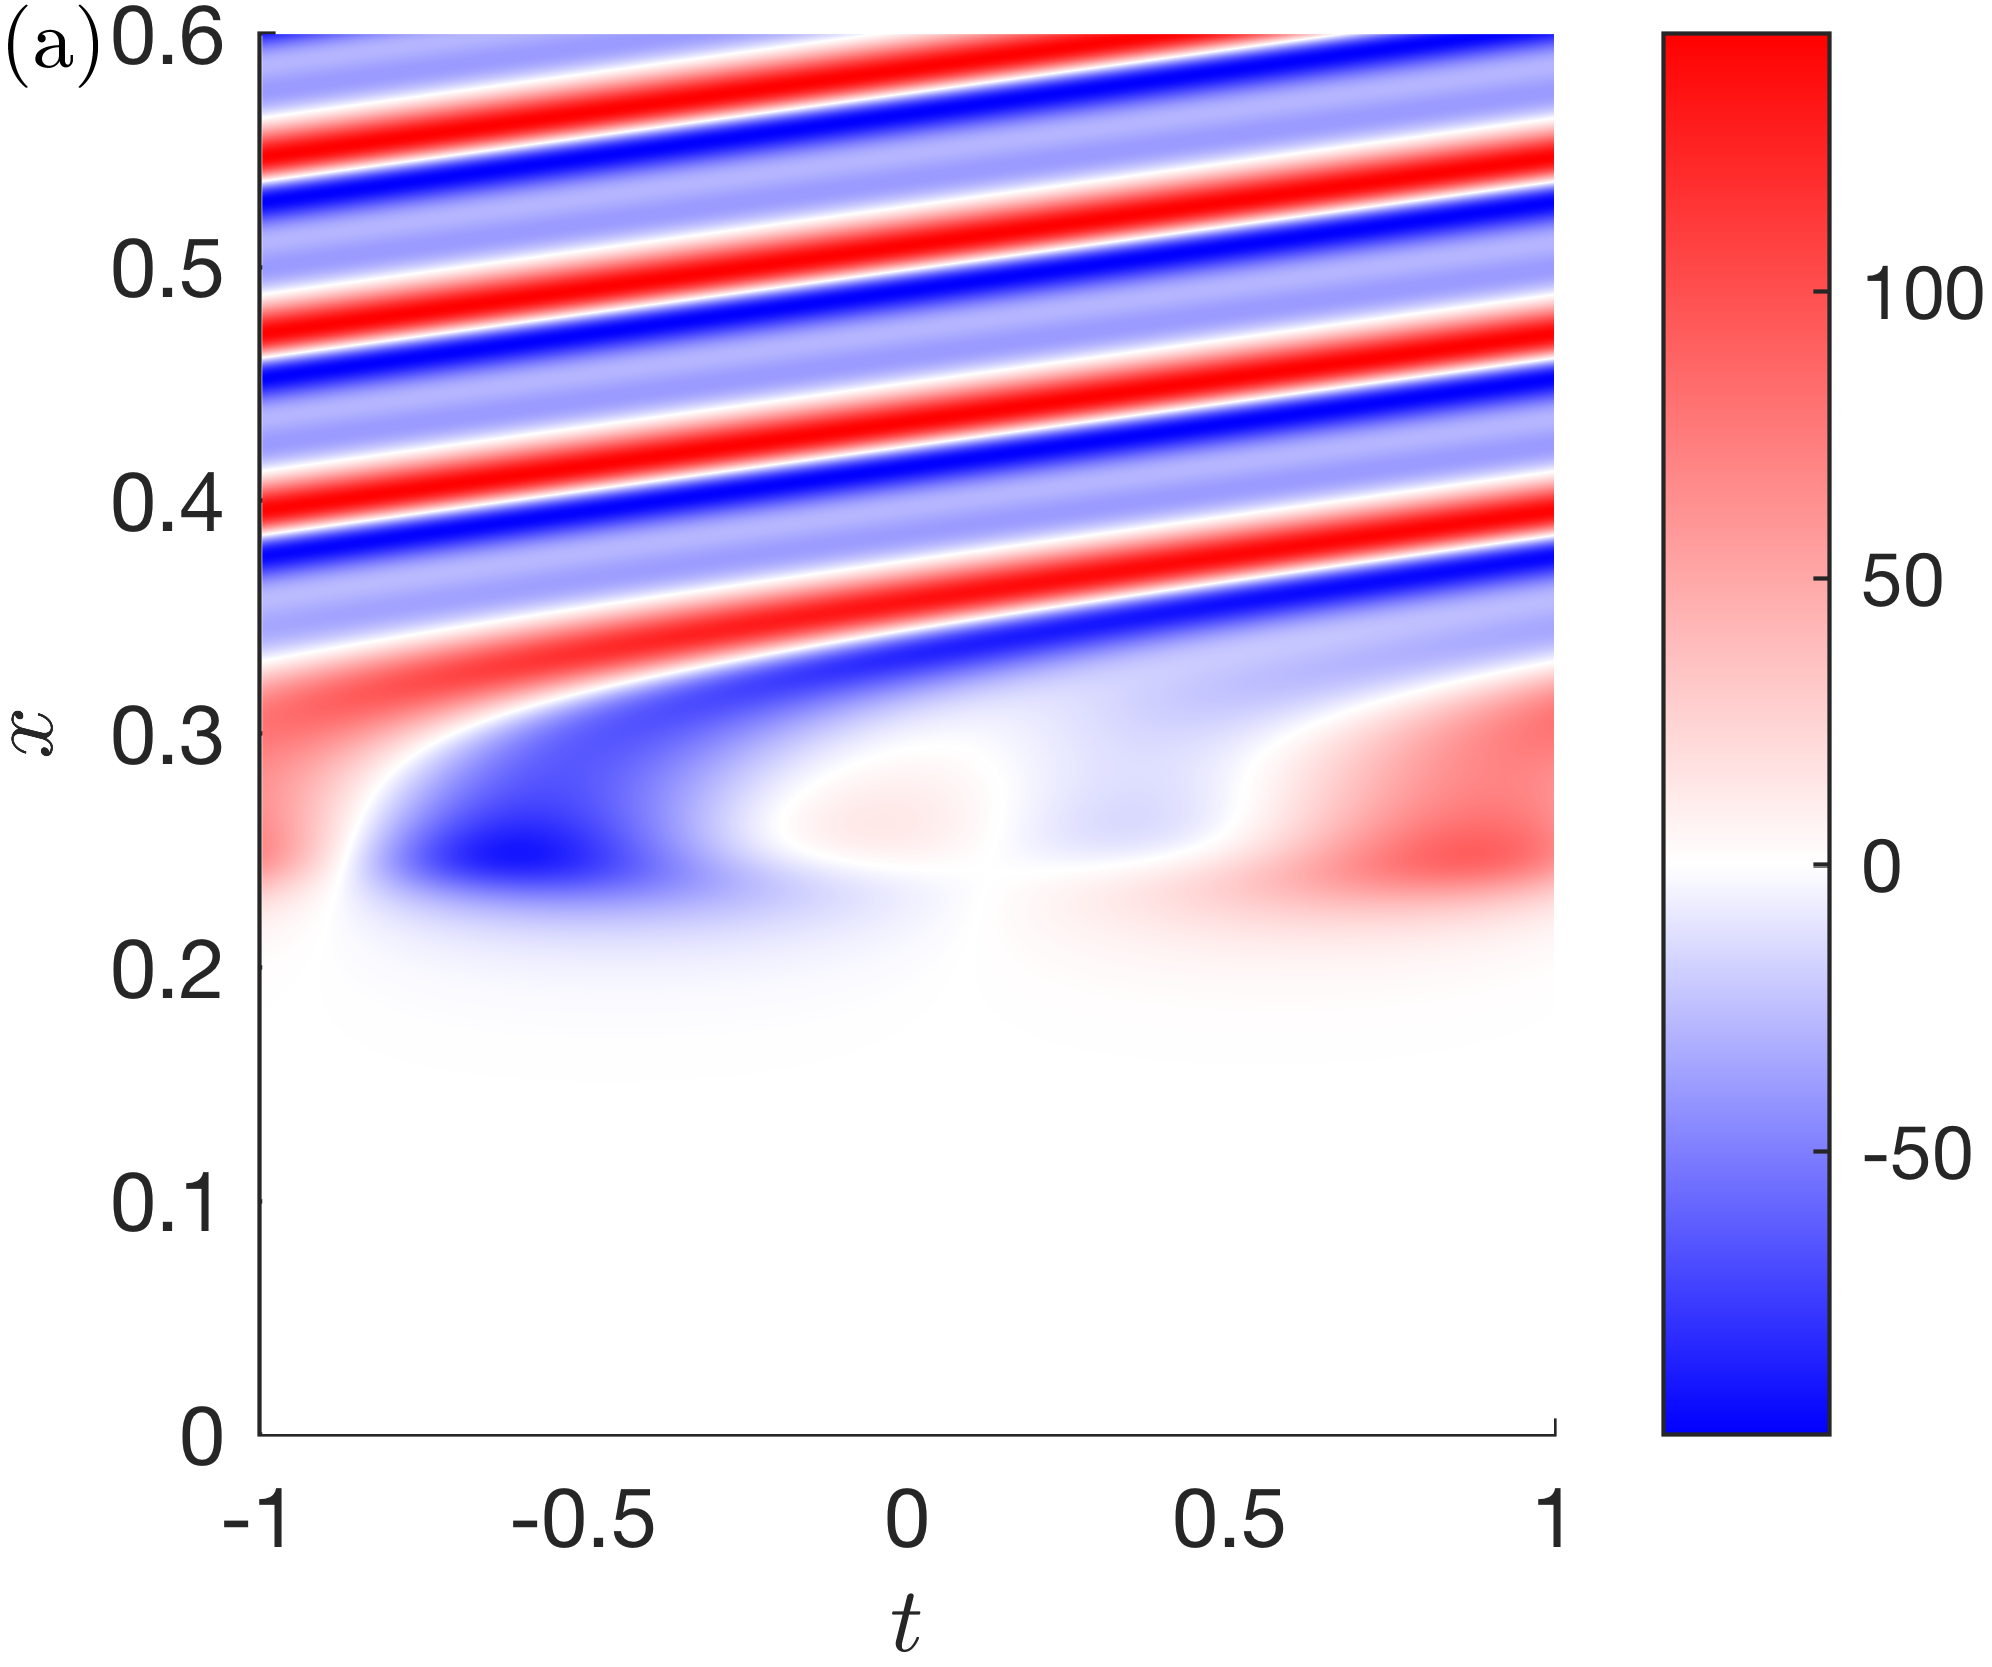
\includegraphics{xt_parallel}
    \hfill
    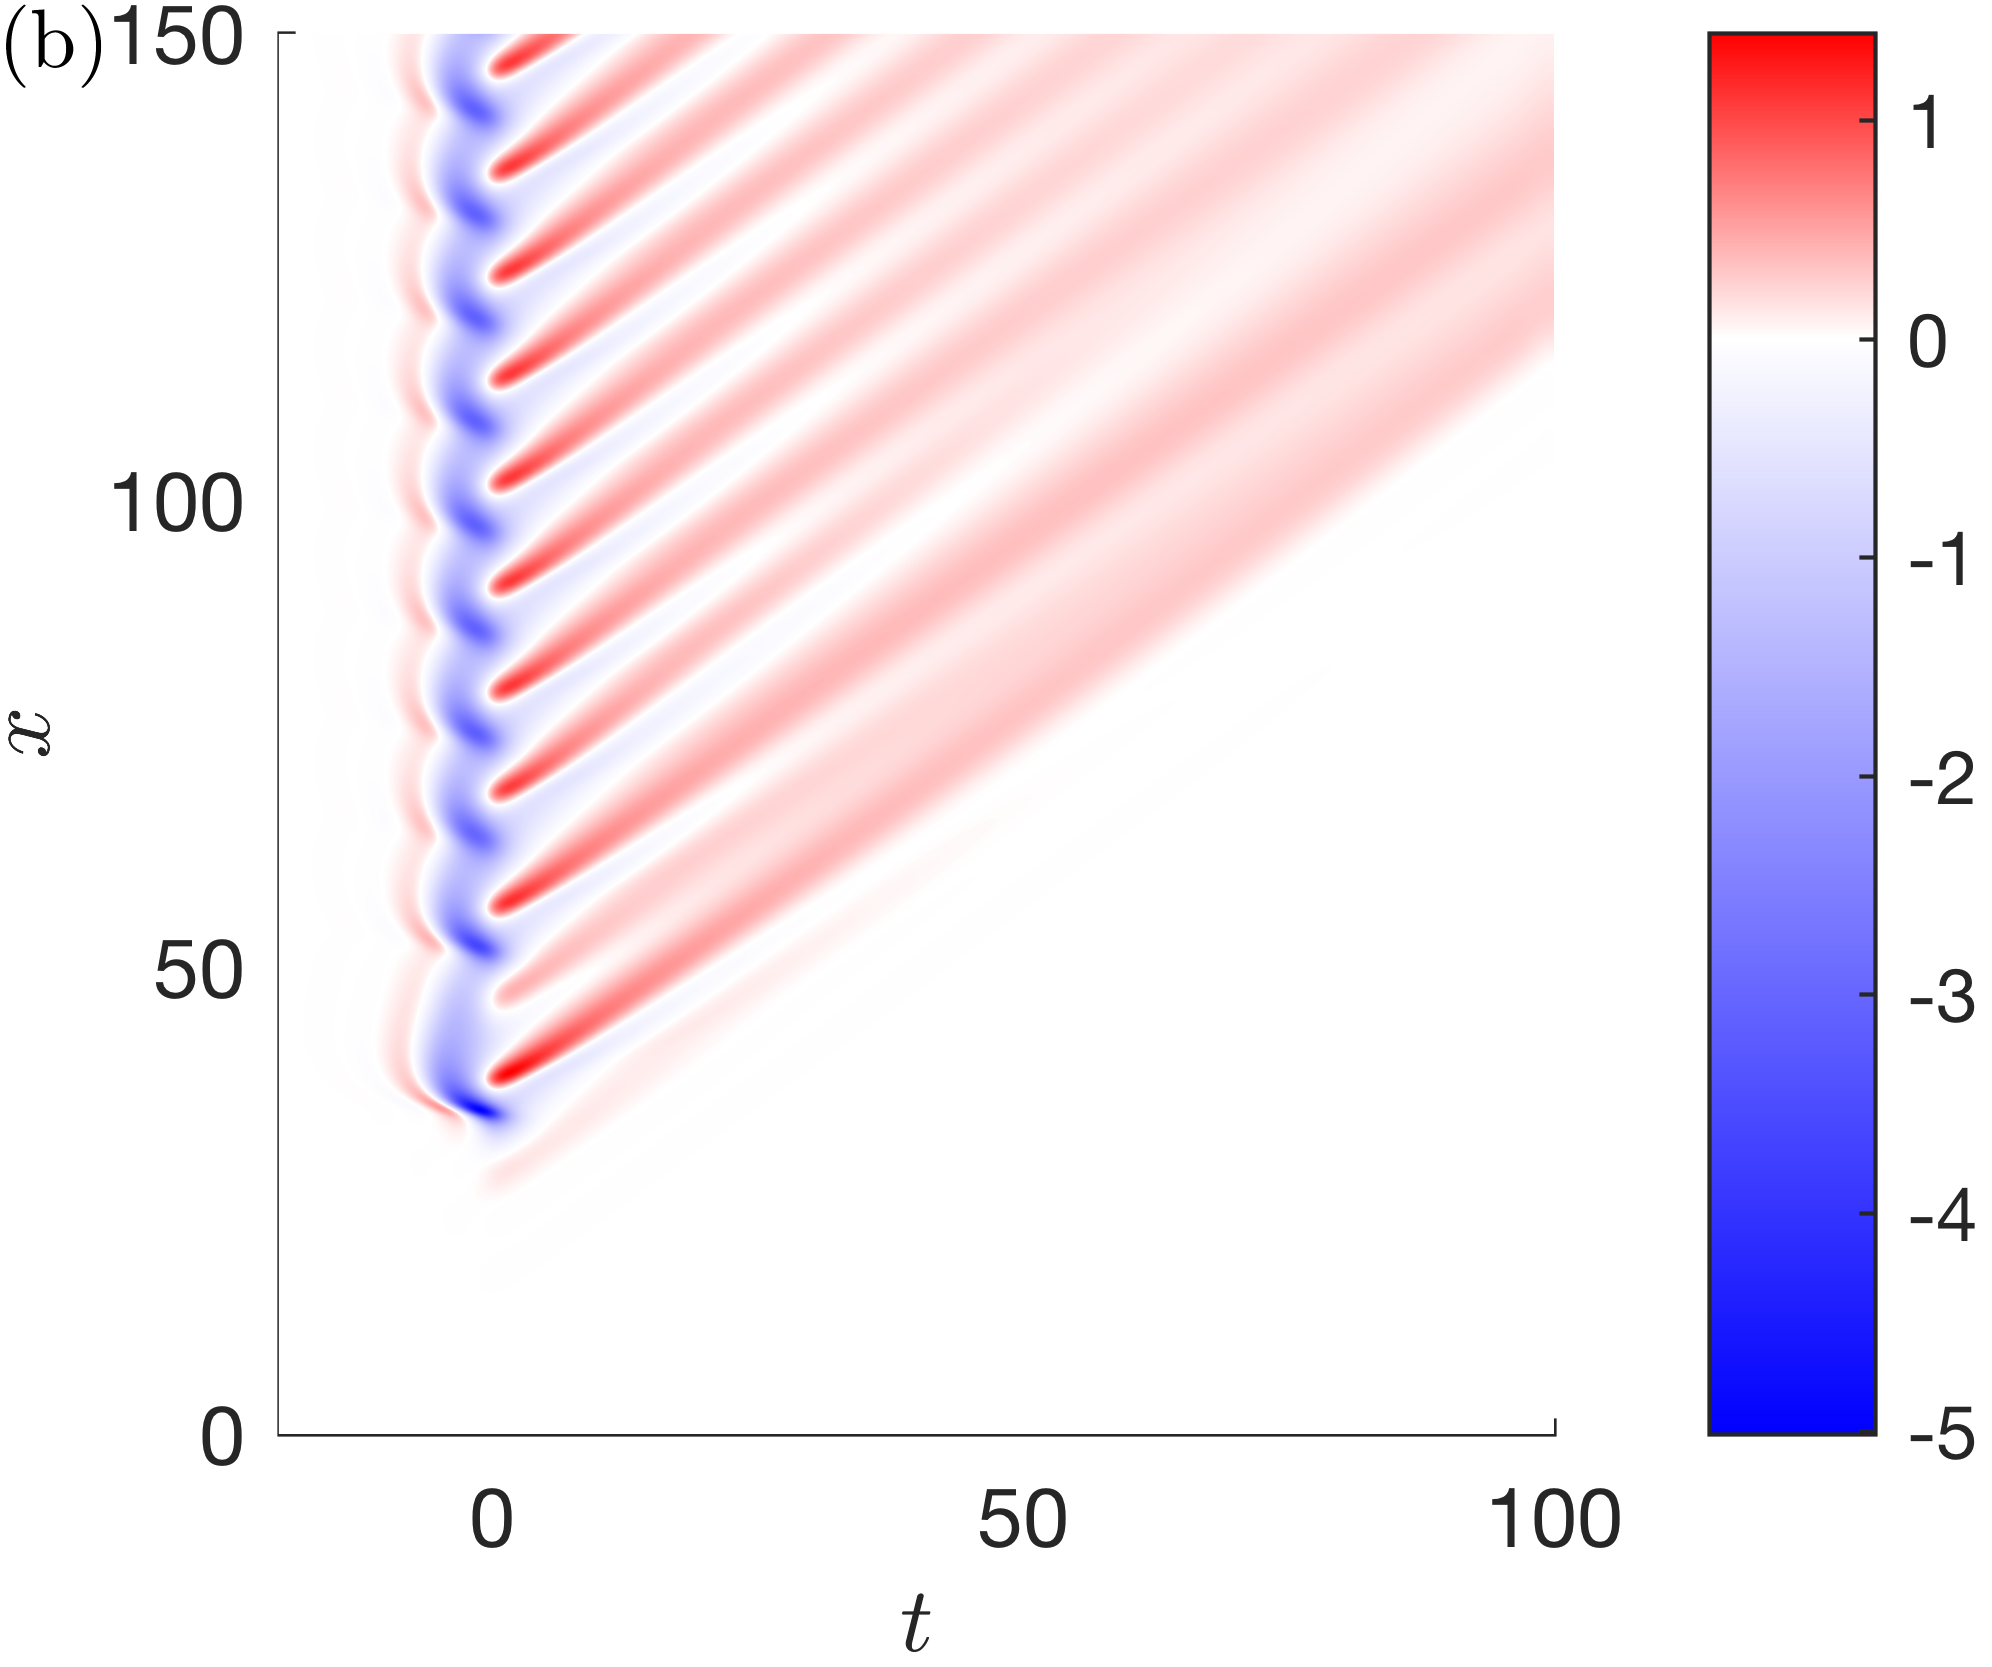
\includegraphics{xt_nonparallel}

    \caption{%
        $x$--$t$ plots of the \KSE, starting from a small random initial condition.
        (a) The parallel equation, with $\mu_0 = \pi^2$ and $\gamma = 0.28$.
        (b) The nonparallel equation, with $\mu_0 = 3.95$ and $\gamma = 1$.%
    }
    \label{fig:time-resolved}
\end{figure}

%======================================================================
%EMMA
%======================================================================
We analyse a variety of different cases but only three different cases will be discussed here, all with the same fixed $\mu = \pi^2$, but with varying $\gamma$. The first case is a point very close to the Hopf stable fixed point, $\gamma = 0.9$, the second looks at a case which is relatively far from the Hopf stability, $\gamma = 0.28$, and finally at a point just before the solution becomes chaotic, $\gamma = 0.24$.  

\begin{figure}[!h]
    \centering
    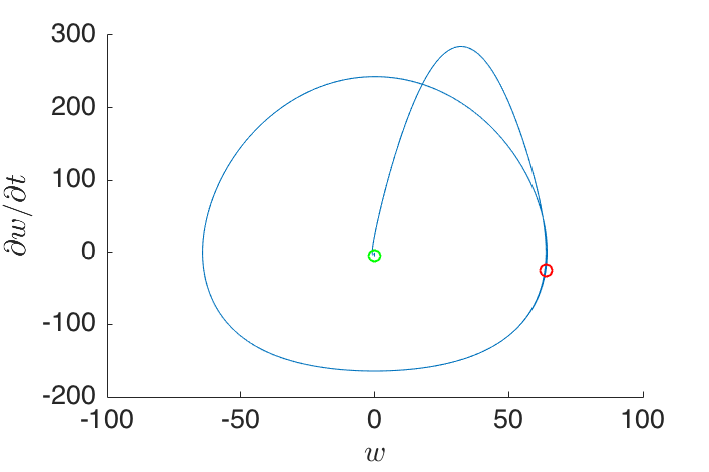
\includegraphics[width=.3\linewidth]{PhasePg09.png}
    \hfill
    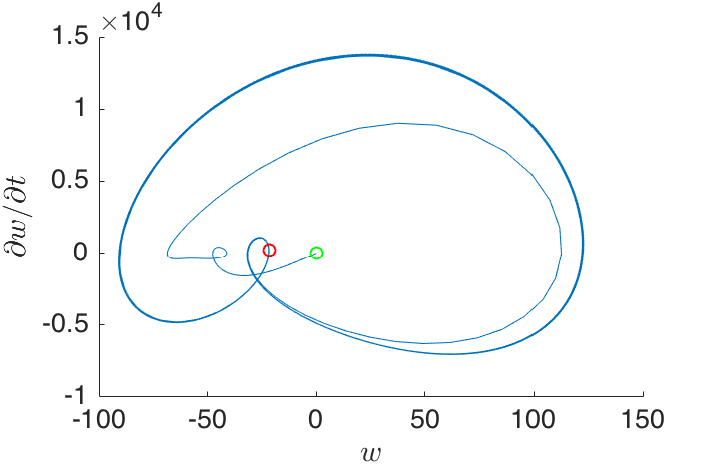
\includegraphics[width=.3\linewidth]{PhasePg028.png}
    \hfill
    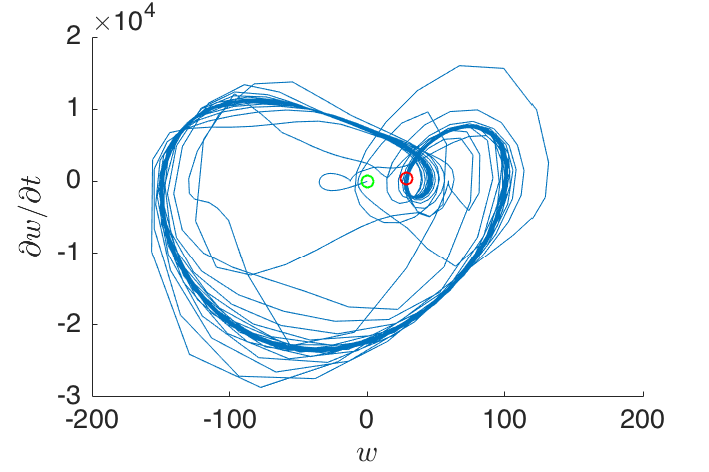
\includegraphics[width=.3\linewidth]{PhasePg024.png}

    \caption{%
        Phase portraits of the three cases for the parallel case. The green spot depicts the inital value and the red depicts the end value.
        (a)  $\mu_0 = \pi^2$, $\gamma = 0.9$.
        (b)  $\mu_0 = 3.95$, $\gamma = 0.28$.
        (c)  $\mu_0 = 3.95$, $\gamma = 0.24$.%  
    }
    \label{fig:parallelPhase}
\end{figure}


\begin{figure}[!h] 
    \centering
    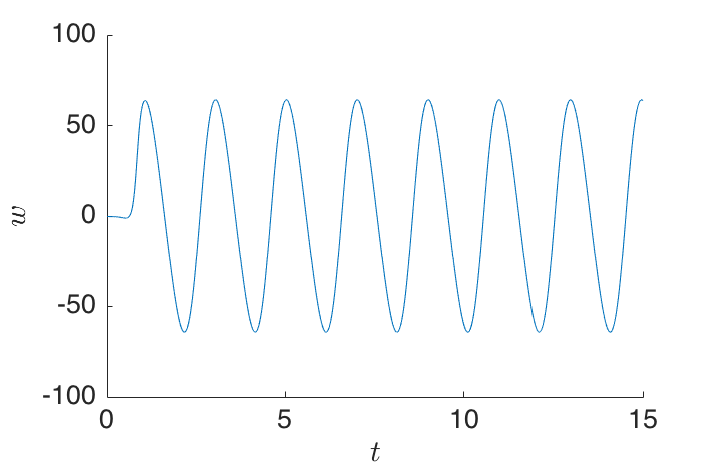
\includegraphics[width=.3\linewidth]{TimeEvo_g09.png}
    \hfill
    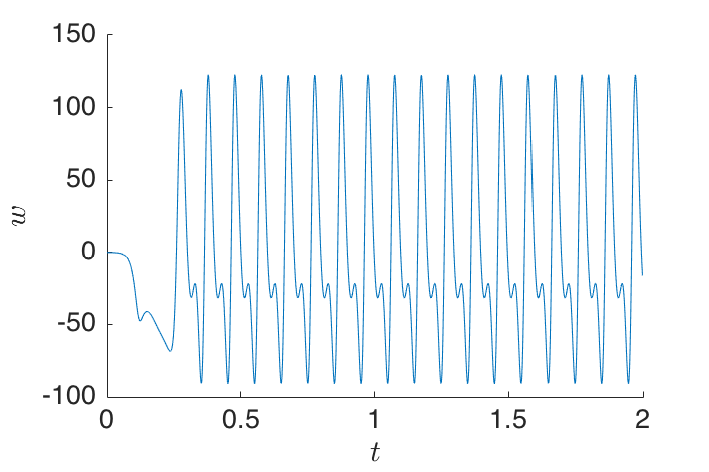
\includegraphics[width=.3\linewidth]{TimeEvo_g028.png}
    \hfill
    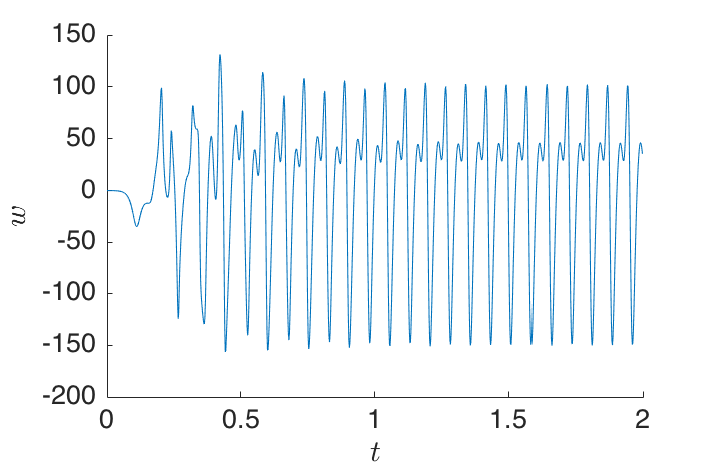
\includegraphics[width=.3\linewidth]{TimeEvo_g024.png}

    \caption{%
        Plots of the solution $w$ with respect to time for the parallel case.
        (a)  $\mu_0 = \pi^2$, $\gamma = 0.9$.
        (b)  $\mu_0 = 3.95$, $\gamma = 0.28$.
        (c)  $\mu_0 = 3.95$, $\gamma = 0.24$.%  
    }
    \label{fig:parallelTime}
\end{figure}

\begin{figure}[!h]
    \centering
    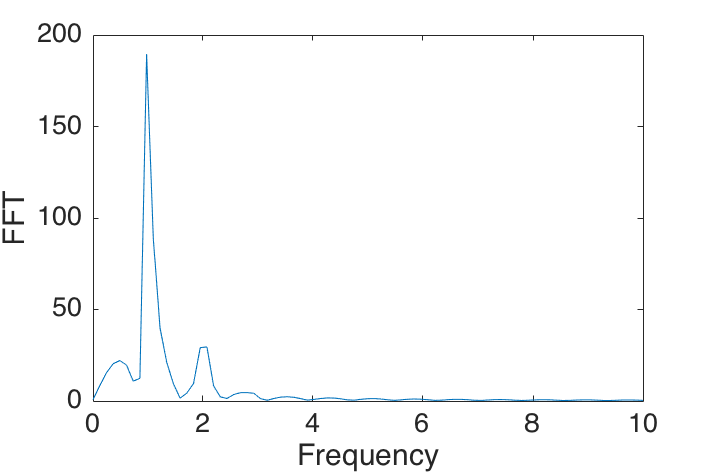
\includegraphics[width=.3\linewidth]{FFT_g09.png}
    \hfill
    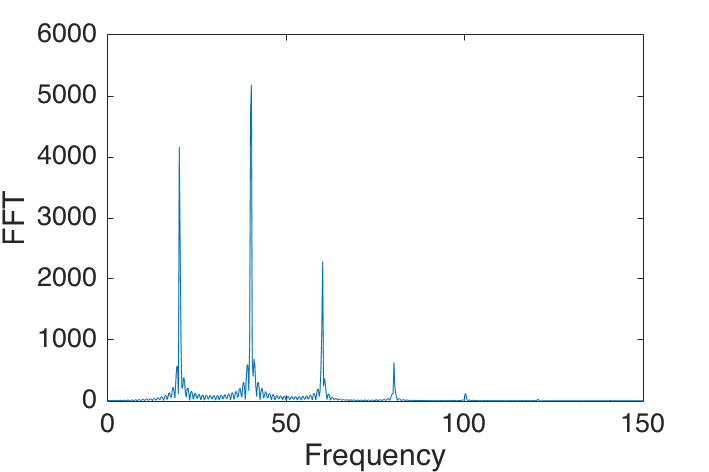
\includegraphics[width=.3\linewidth]{FFT_g028.png}
    \hfill
    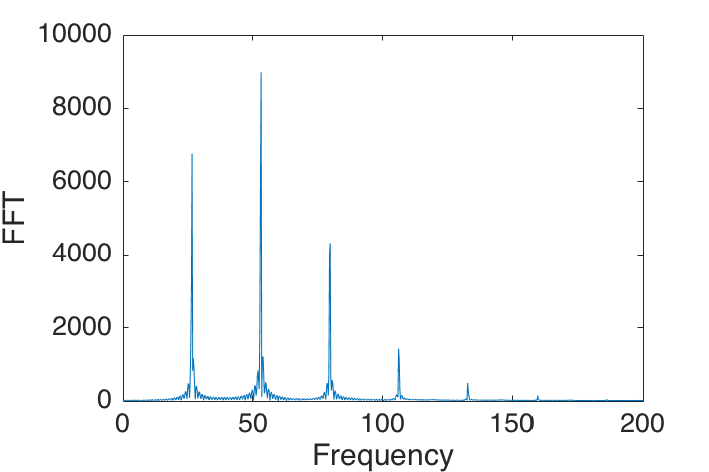
\includegraphics[width=.3\linewidth]{FFT_g024.png}

    \caption{%
        Plots for the fast fourier transform of the solution in time for the parallel case.
        (a)  $\mu_0 = \pi^2$, $\gamma = 0.9$.
        (b)  $\mu_0 = 3.95$, $\gamma = 0.28$.
        (c)  $\mu_0 = 3.95$, $\gamma = 0.24$.%  
    }
    \label{fig:parallelFFT}
\end{figure}

The phase portraites vary largely for the different points, with case(a) depicting a periodic limit cycle, whereas cases (b) and (c) both show a quasi-periodic limit cycle, see figure(\ref{fig:parallelPhase}). Any value of gamma satisfying $?<\gamma<1$ produces phase plots similar to that of case (a), any satisfying $0.24<\gamma<?$ will produce a plot similar to (b) and any with $\gamma<0.24$ exhibit chaos.\eec{find out at which point we begin to see a change from one state to the next} Interestingly, case (c) appears to have a change in phase just before the solution becomes chaotic. 

Case $\mu_0 = \pi^2$ and $\gamma = 0.9$ has the longest transient and as we move further away from the supercritial hopf bifurcation this transient region exists for shorter time periods, shown in figure (\ref{fig:parallelTime}).  This is to be expected since the case (a) is the closest to the supercritial hoph bifurcation and the cases selected increase in distance from the fixed point. From these set of figures we can see that the limit cycle for $\gamma = 0.9$ exibits a very regular, almost sinusoidal profile. This is confirmed by the fast Fouier transform which shows an extremely strong primary frequency, figure(\ref{fig:parallelFFT}a). As we progress further away from the fixed point to the quasi-periodic orbits we can see more and more non-linear dynamics present in the figures (\ref{fig:parallelTime}) and (\ref{fig:parallelFFT}) which would explain the quasi-periodic orbits in the phase portraits we see. 



%=======================================================================
%END EMMA
%=======================================================================

\subsection{Non-parallel equation}

\autoref{fig:time-resolved}(b) depicts\ldots

\section{POD-DEIM models of the K-S equation}
\label{sec:pod-deim}
The ability of the POD-DEIM modes to capture the dynamic of the K-S equation through a Reduced Order Model (ROM) is investigated. Not only do we see that a small number of modes well capture the limit cycle, but also that transient modes correctly capture the limit cycle dynamics, and limit cycle modes correctly capture transient dynamic. We specify that the transient modes (TM) refer to the POD-DEIM modes computed from the temporal snapshots of the transient part of the DNS while limit cycle modes (LCM) refer to the POD-DEIM modes computed from the temporal snapshots of the limit cycle part of the DNS. These definitions are case dependant, so we specify the time ranges for the different dynamics inside each following subsections. 

\subsection{Parallel equation}
\label{subsec:parallel}
The POD-DEIM modes and ROM of the parallel equation are based on a Fourier pseudospectral discretization. We investigate two sets of parameters, $\gamma = 0.9$ , $\mu=\pi^2$, $U=1$ and $\gamma = 0.28$ , $\mu=\pi^2$, $U=1$. The dynamic of this system for both sets of parameters represents a limit cycle in the Hopf bifurcation sense when considering $\gamma$ as bifurcation parameter. The first set is close to the instability threshold and the second set is further away from it, where nonlinear effects become stronger and strengthen the second harmonic of the Fourier spectrum, see \kkc{figure \ref{spectrum}}.

The ROMs computed from the POD-DEIM modes of the limit cycle converge when a minimum of 8 modes, for the first set, and 10 modes, for the second set of parameters, are considered. As expected, the accuracy of the ROM increases with the number of modes, see Table \ref{tab:errorcycle}. The errors are a shift in the convective velocity and a mismatch in the amplitude of the limit cycle. 

\begin{table}[!ht]
\begin{center}
\begin{tabular}{ c || c | c | c | c | c |c|}
%\hline
 N of modes &  8 & 10 & 12 & 14 & 18 &30\\ \hline
ROM error $\gamma=0.9$, &  \multirow{2}{*}{$3\cdot 10^{-2}$} & \multirow{2}{*}{$5\cdot 10^{-4}$} & \multirow{2}{*}{$9\cdot 10^{-5}$} & \multirow{2}{*}{$7\cdot 10^{-5}$}& \multirow{2}{*}{$4\cdot 10^{-5}$}& \multirow{2}{*}{$1\cdot 10^{-5}$}\\
 $\mu = \pi^2$, $ U = 1$ & & & & && \\ \hline
ROM error $\gamma=0.28$, & \multirow{2}{*}{-}  & \multirow{2}{*}{$1\cdot 10^{0}$}  & \multirow{2}{*}{$3\cdot 10^{-2}$}  & \multirow{2}{*}{$9\cdot 10^{-3}$}& \multirow{2}{*}{$1\cdot 10^{-4}$}& \multirow{2}{*}{$1\cdot 10^{-4}$} \\
 $\mu = \pi^2$, $ U = 1$ & & & & &&\\
\hline
\end{tabular}
\caption{Relative errors of the ROM for the parallel case with respect to the DNS on 10 limit cycles.\label{tab:errorcycle}}
\end{center}
\end{table}

The ability to reproduce the transient dynamic by the ROM built on the limit cycle modes is investigated for the second case, $\gamma=0.28$, $\mu_0=\pi^2$, $U=1$. The number of modes is fixed to 30 to avoid any mismatches between the ROM and the DNS along the limit cycle. The solutions obtained from the DNS and ROM and their energies are depicted in Fig. \ref{fig:Energyparallel} (a) and (b). 
\begin{figure}
    \centering
    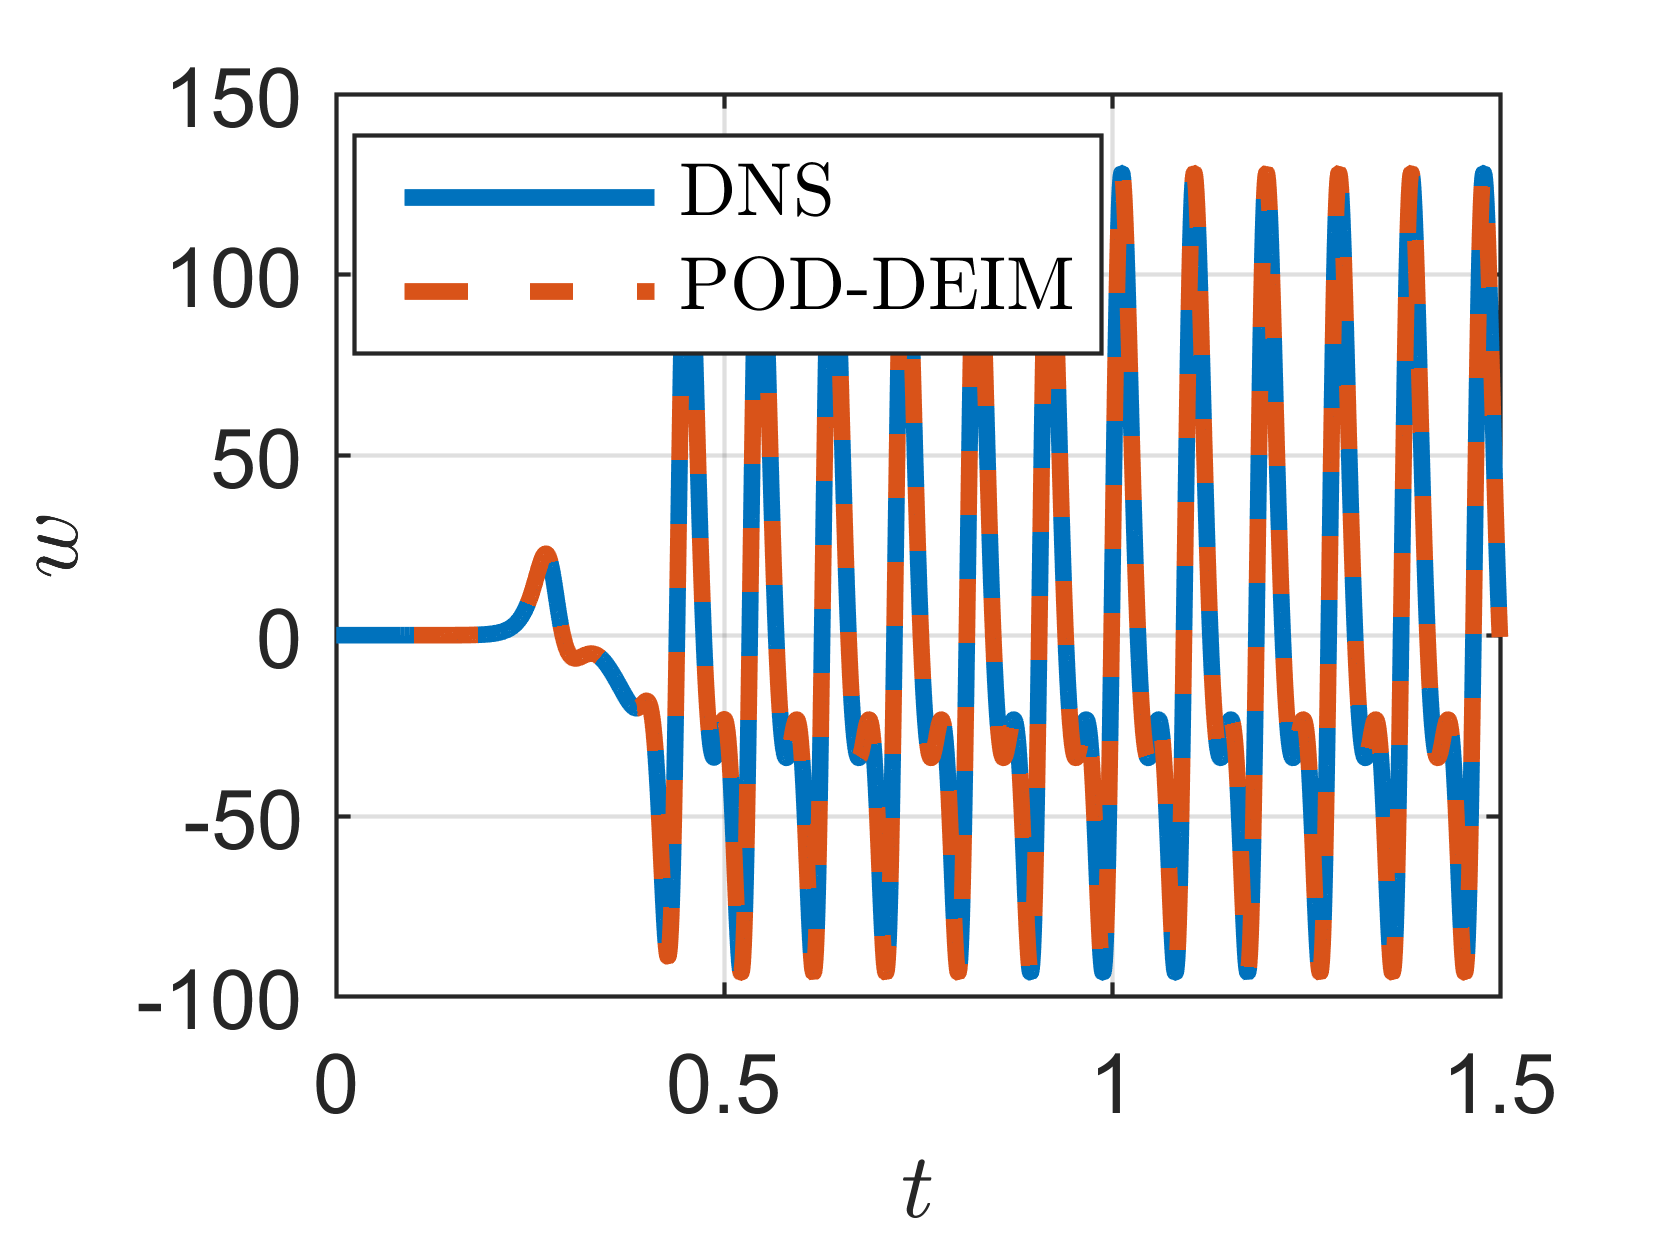
\includegraphics{TimeEvoparallel}
    \hfill
    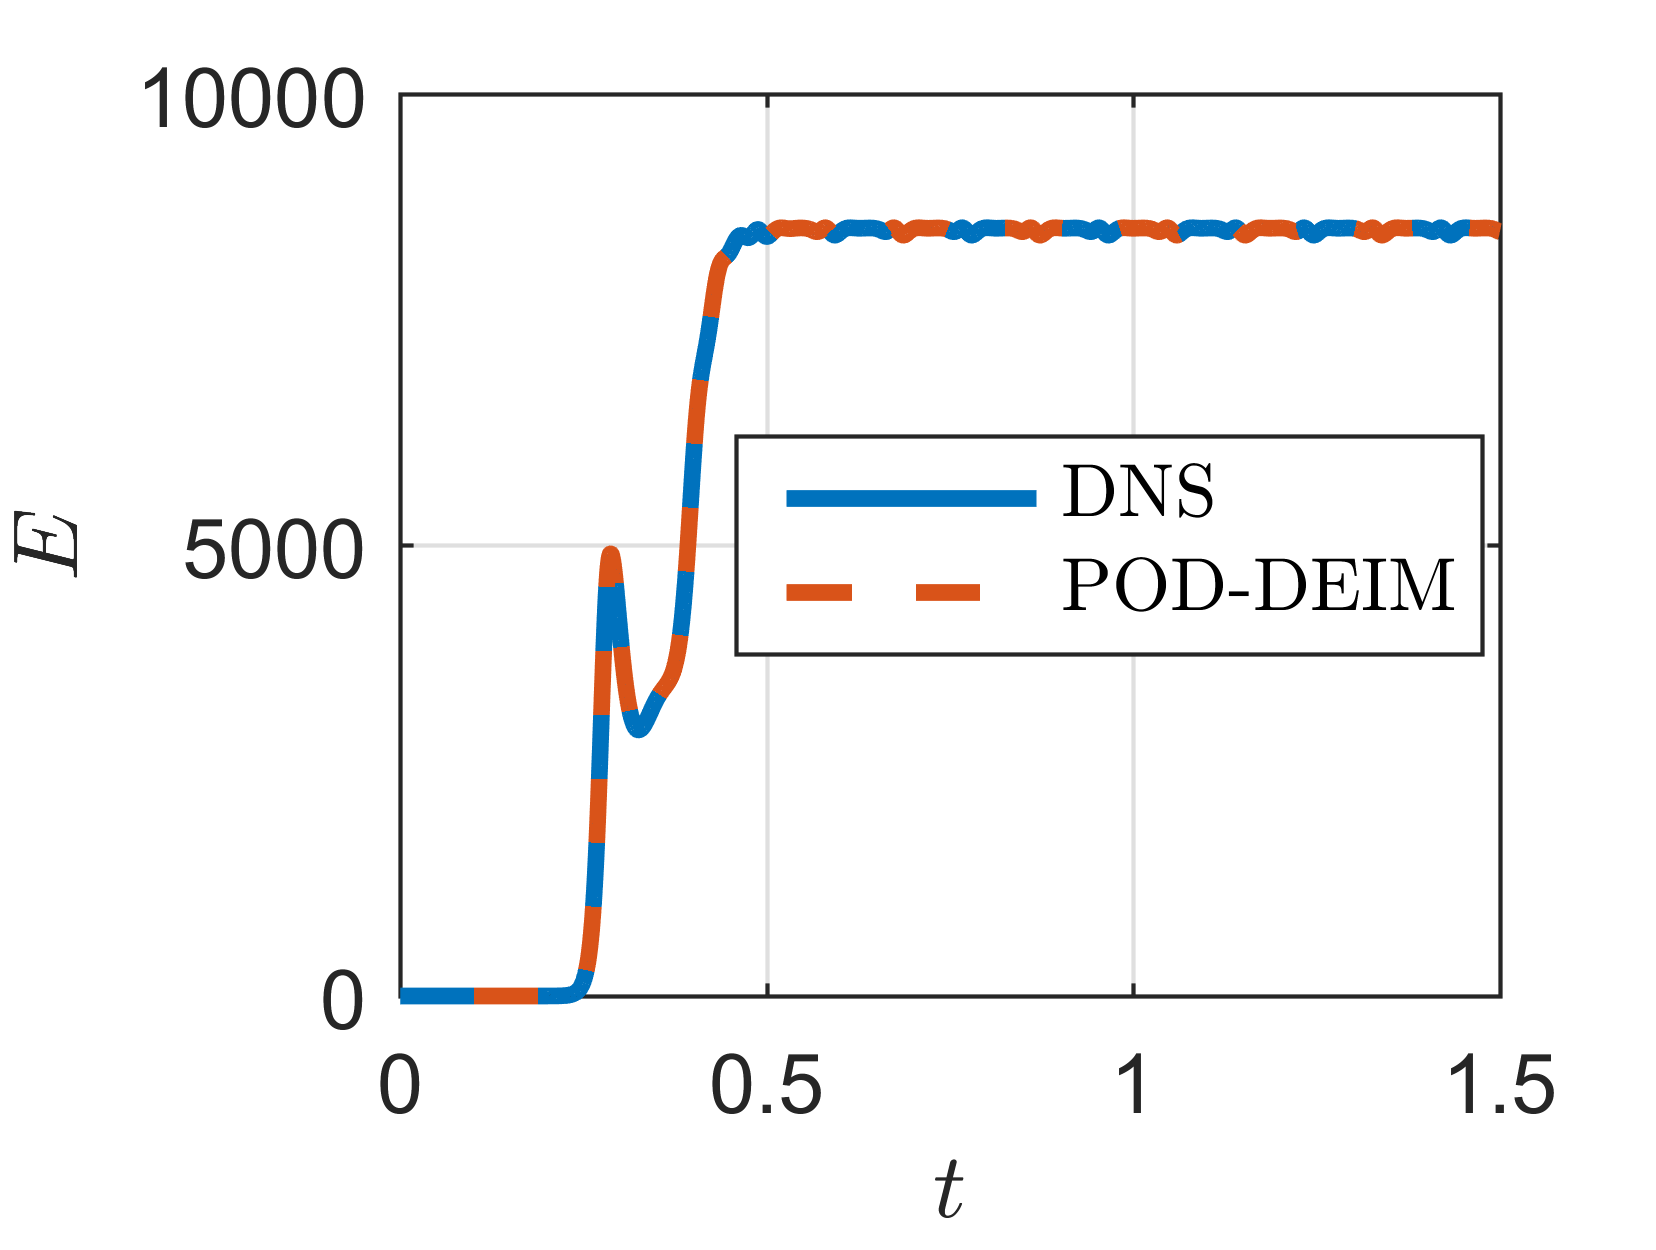
\includegraphics{Energy3}
    \caption{%
    	    (a) Time history of the ROM (red) and DNS (blue) with $\mu_0 = \pi^2$ and $\gamma = 0.28$, where the ROM is built on the limit cycle modes computed for $t\in [0.5, 1.5]$ and evaluated in the transient regime, starting at $t=0.1$.
        (b) Energy of the ROM and DNS solutions for the same conditions.
    }
    \label{fig:Energyparallel}
\end{figure}
The time evolution as well as the energy of the signal are in agreement, a relative error less than $5 \cdot 10^{-5} $ is obtained. These results show that the POD basis, computed for $t\in [0.5, 1.5]$, is able to capture the DNS evolution out of its range of definition. Any spatial solutions from the DNS snapshots projected in the POD basis are identical and may be used as initial conditions without any deviation in the time evolution of the DNS with the ROM. Thus not only does the POD basis cover all the DNS solution but also, the dynamic of the transient part of the DNS is captured. The figure of the reverse approach is not presented, the prediction of the limit cycle by the transient modes, returns the same accurate results. This means that the POD basis from the limit cycle, computed for $t\in [0.5, 1.5]$, and the one from the transient part, computed for $t\in [0.1, 0.5]$, represents the same subspace with different eigenmodes, Fig \ref{fig:PODmodeparallel}, and that the POD-DEIM method faithfully reproduce the dynamic of the system. 
\begin{figure}
    \centering
    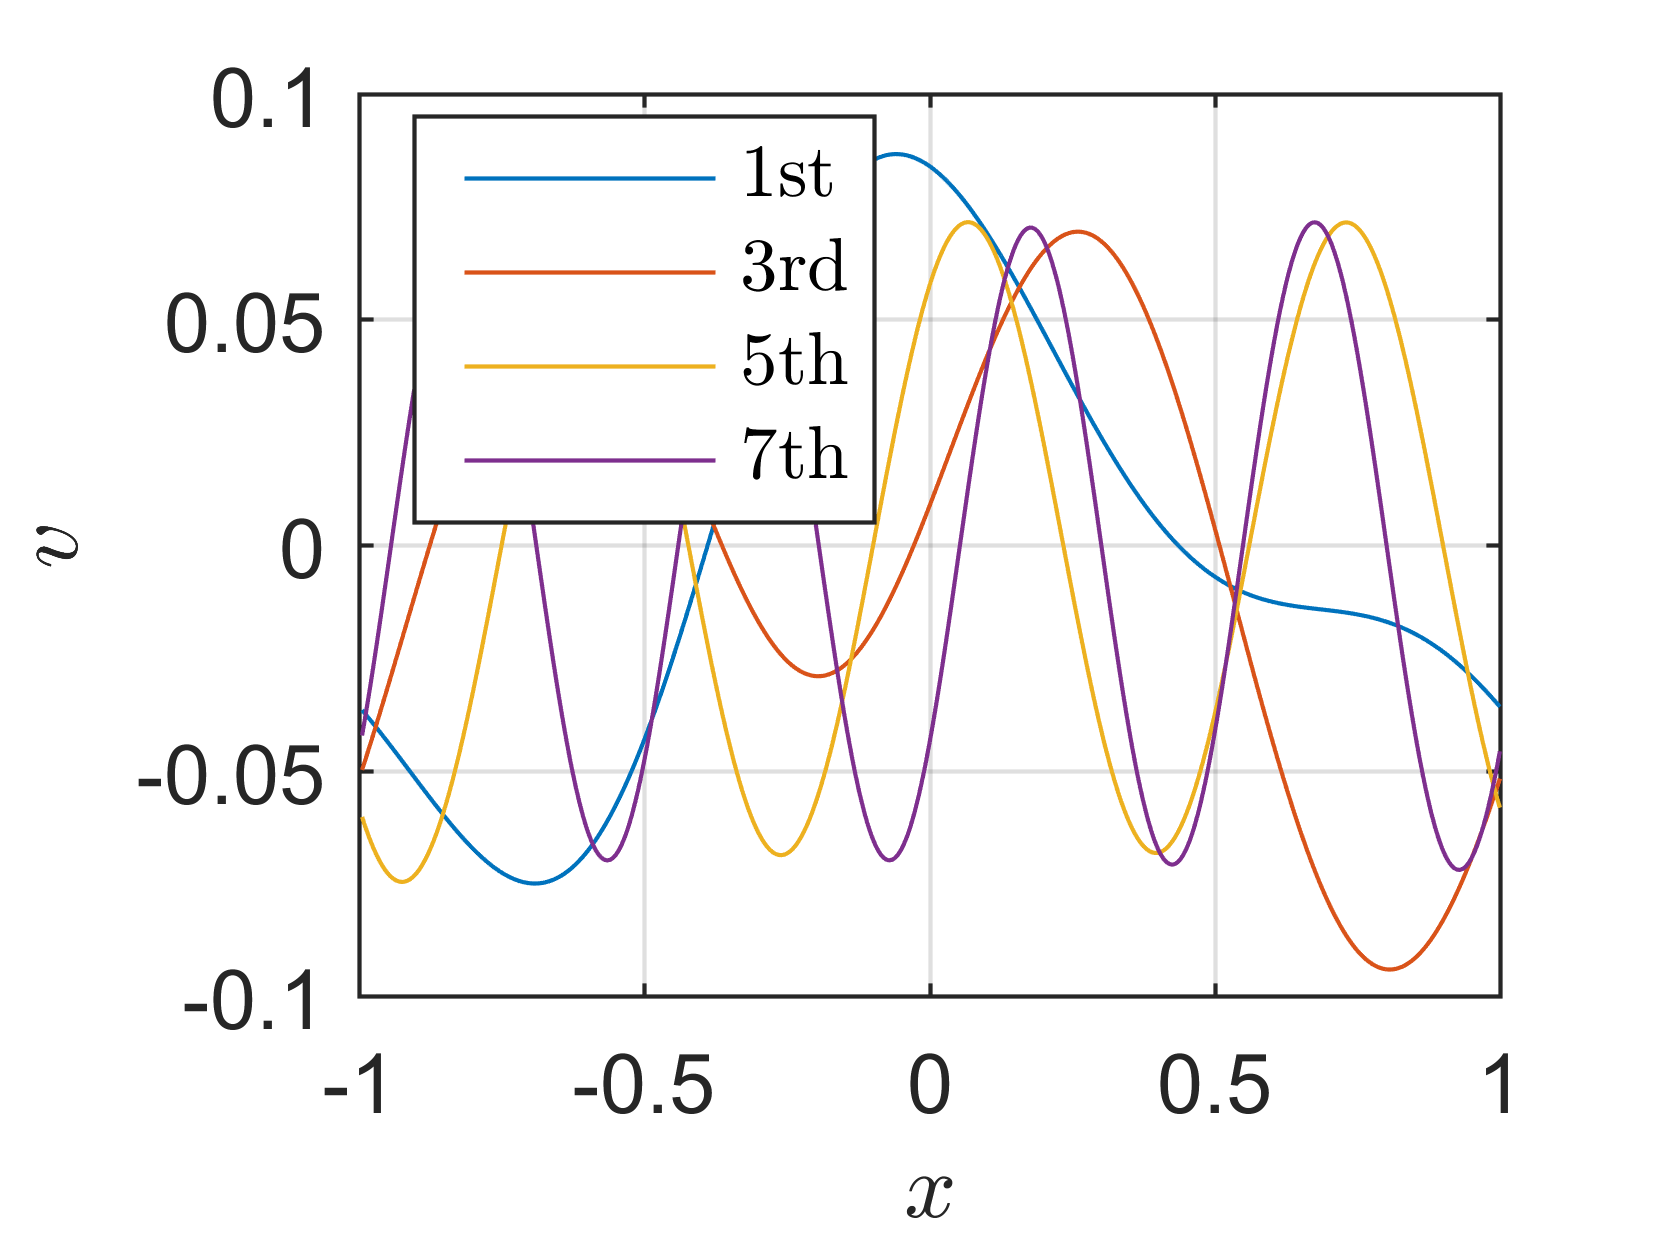
\includegraphics{PODMode1}
    \hfill
    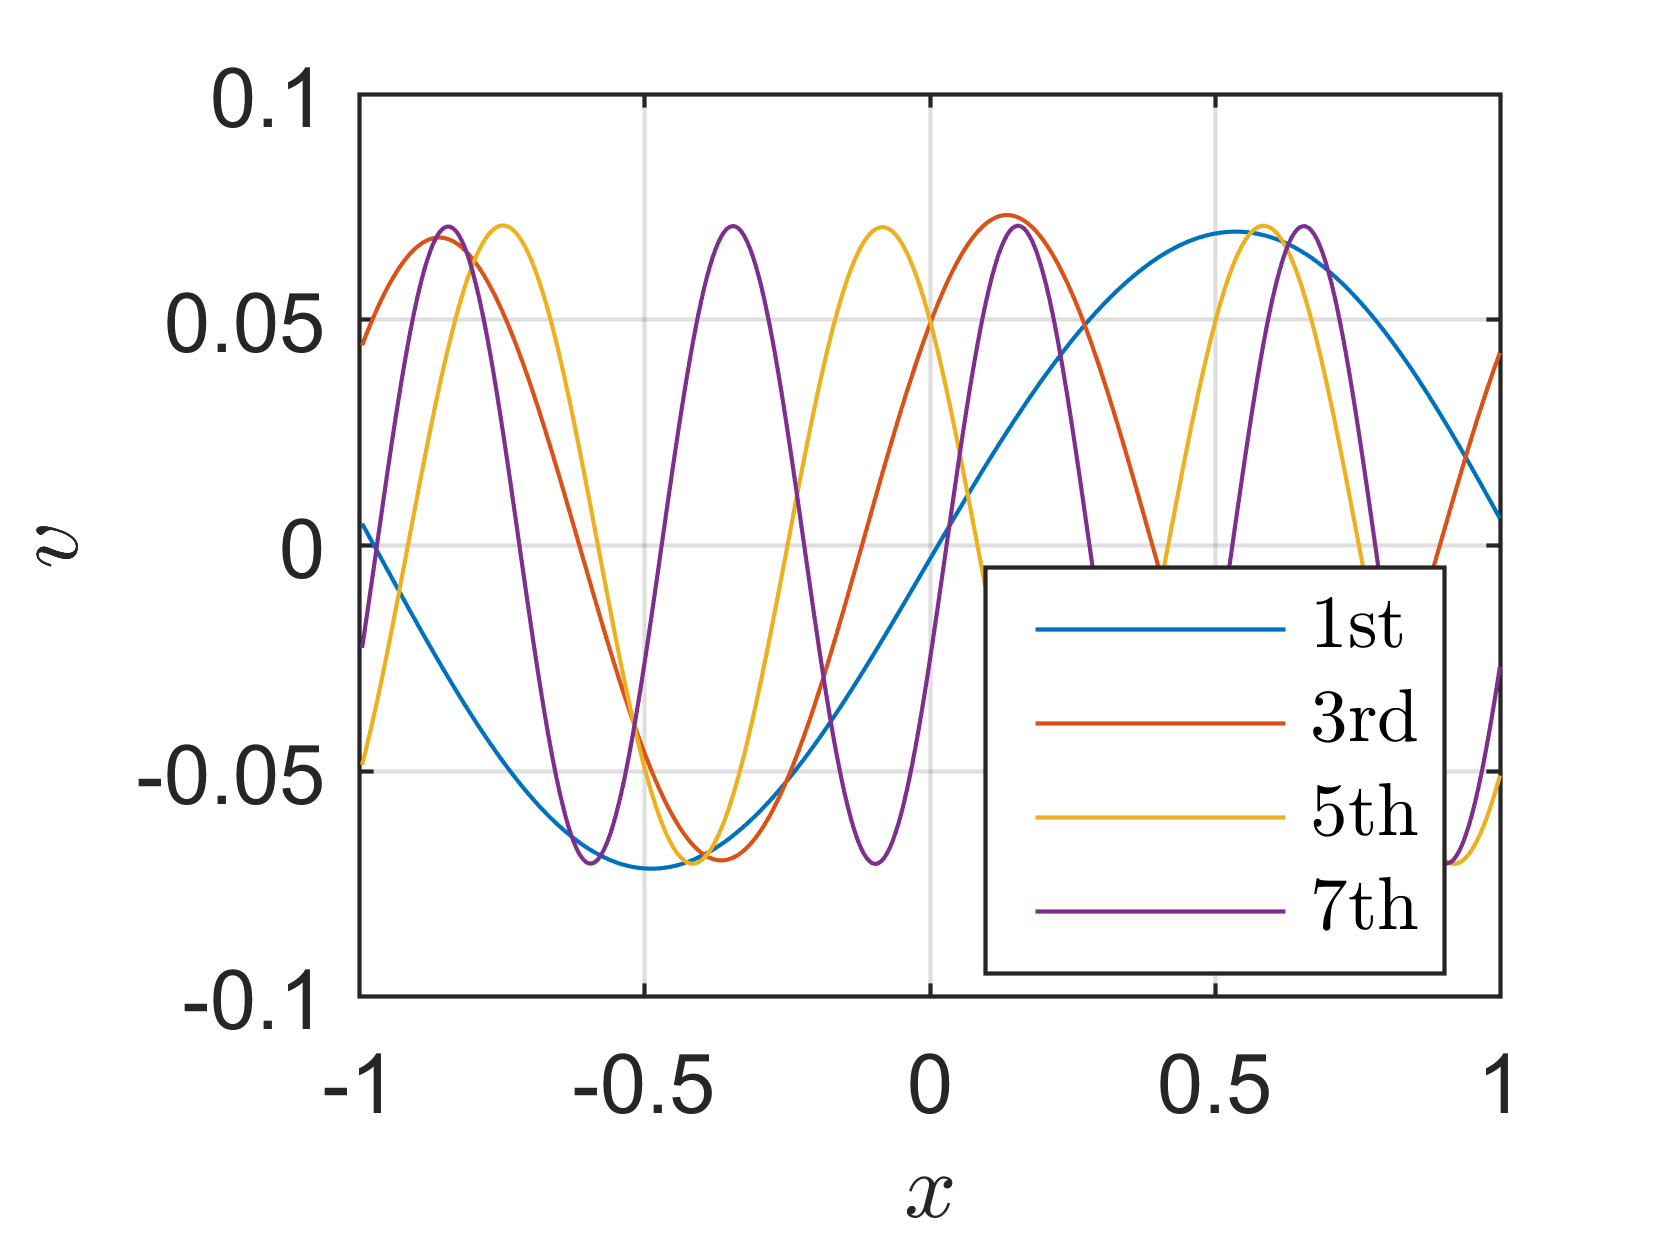
\includegraphics{PODMode2}
    \caption{%
    	    (a) POD modes for  $\mu_0 = \pi^2$ and $\gamma = 0.28$ built on the transient regime for $t\in [0.1, 0.5]$.
        (b) POD modes for  $\mu_0 = \pi^2$ and $\gamma = 0.28$ built on the limit cycle regime for $t\in [0.5, 1.5]$.
    }
    \label{fig:PODmodeparallel}
\end{figure}

The solution of the parallel case involved a convective wave in a periodic domain, which by definition is spatially invariant. Thus the space preferences of the DEIM modes, which are located at the underly nonlinearities of the dynamics are  scattered throughout the domain. This property of the problem may the construction of different basis which has the same subspace and allow us to peak any collection of DNS snapshots to reproduce the dynamic of the system with a ROM based on POD-DEIM.      

\subsection{Nonparallel equation}
\label{subsec:nonparallel}
The nonparallel K-S equation is discretized by finite element in the domain $x \in [-100,100]$. The parameters are set to $\mu = 3.95$ , $\gamma=1.0$ and $U=1$. This dynamical system, for this set, has only one unstable complex conjugate eigenvalue which leads to a Hopf bifurcation. The dynamic of the nonparallel K-S equation is localized around $x=0$ where waves appear and are convected downstream. The POD-DEIM modes built on the limit cycle $t\in[100,200]$, reveal that the POD modes, Fig \ref{fig:PODmodenonparallel} (a), extend to the end of the domain. 
\begin{figure}
    \centering
    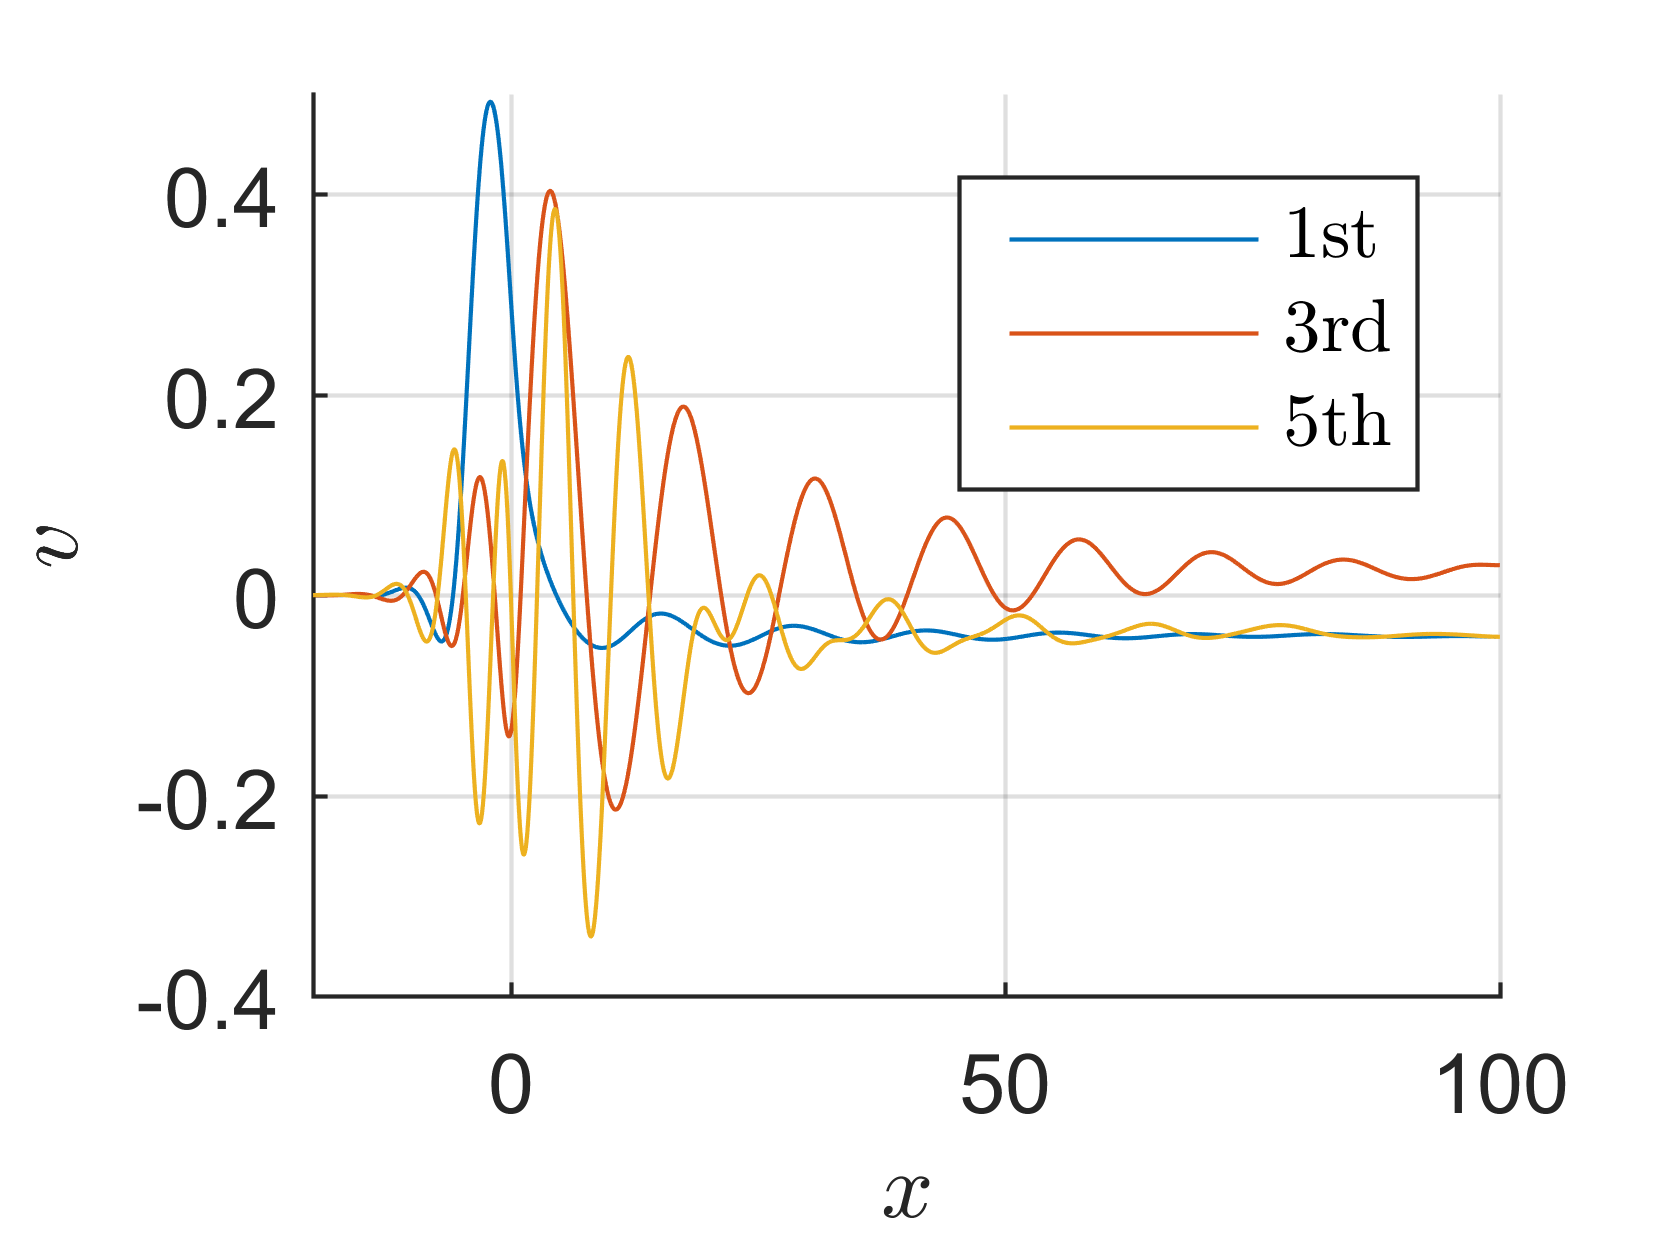
\includegraphics{PODModenon}
    \hfill
    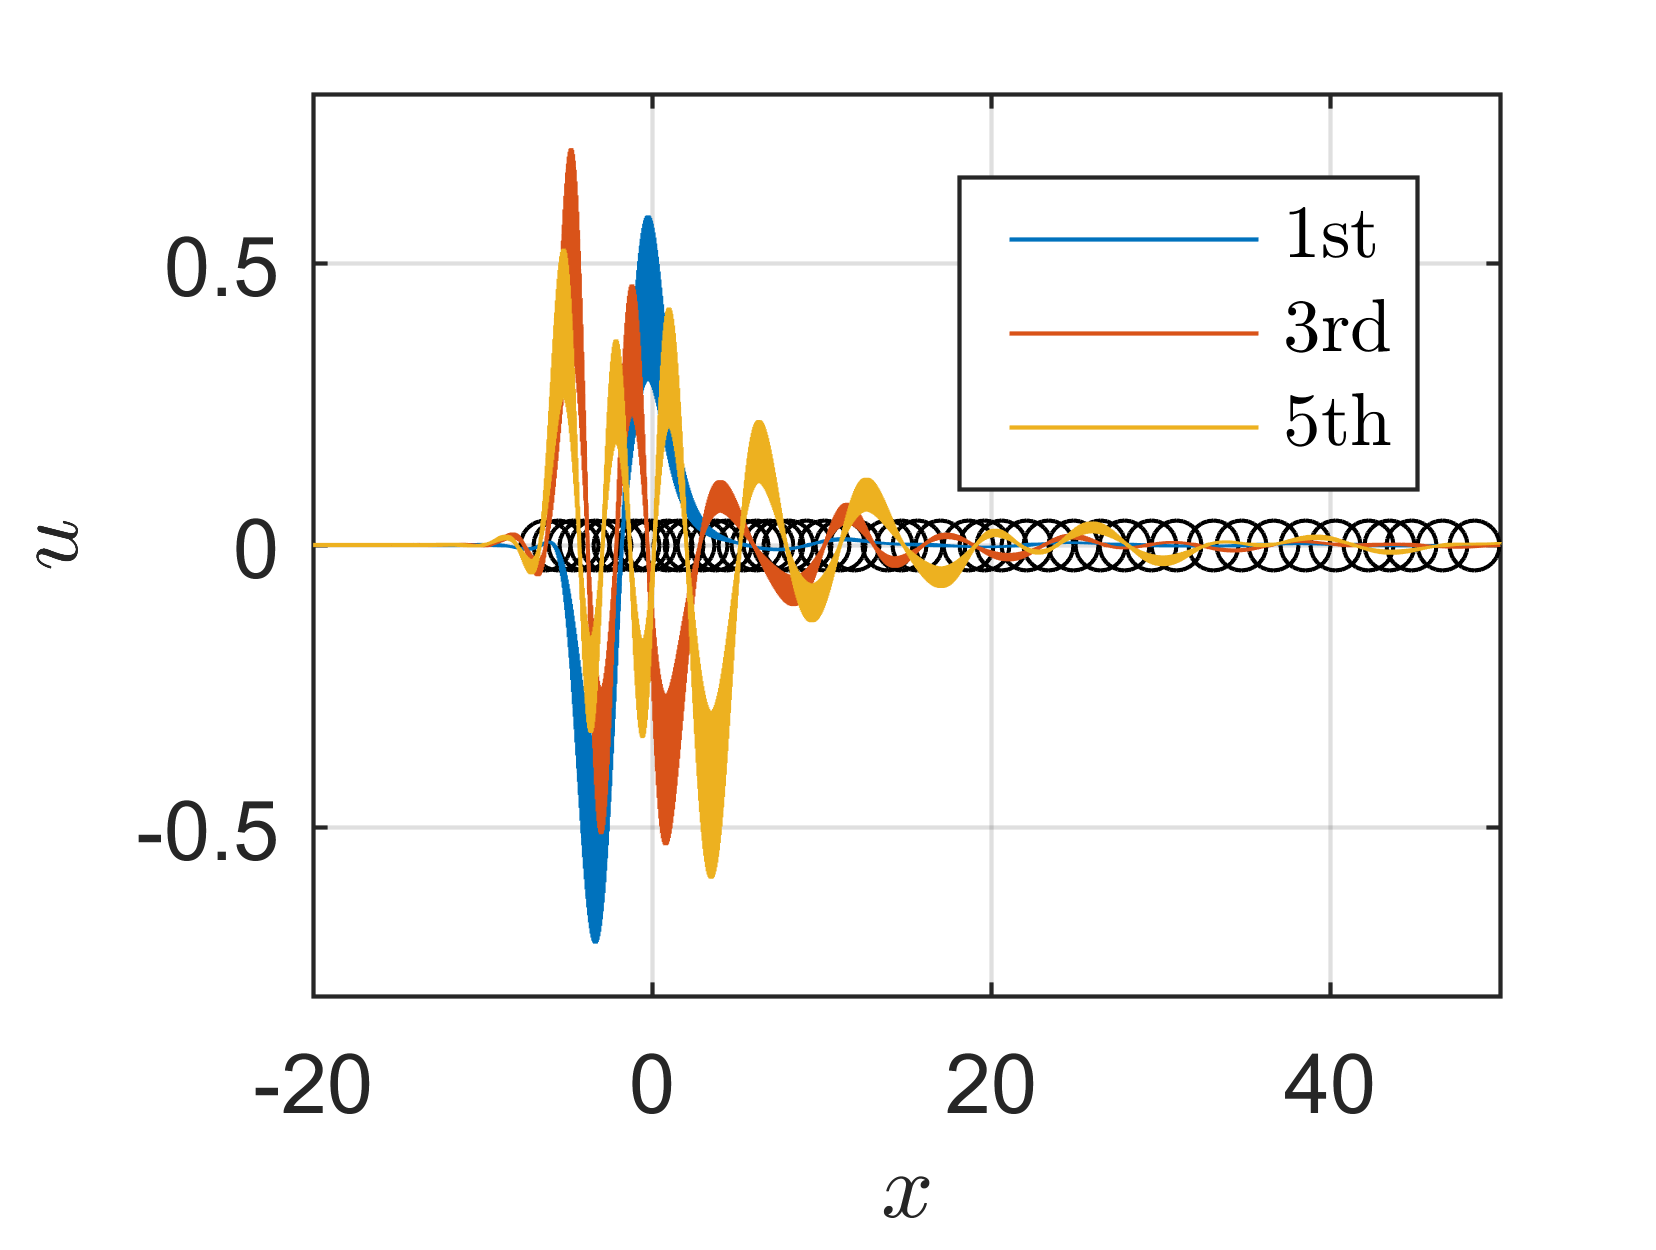
\includegraphics{DEIMModenon}
    \caption{%
    	    (a) POD modes and (b) DEIM modes for  $\mu_0 = 3.95$ and $\gamma = 1.0$ built on the limit cycle regime for $t\in [100, 200]$ and the 70 location of the DEIM points.
        }
    \label{fig:PODmodenonparallel}
\end{figure}
In contrast to the parallel case where spatial invariance appears, the DEIM modes, Fig \ref{fig:PODmodenonparallel} (b), are gathered around the center of the domain. Figure \ref{fig:PODmodenonparallel} (b) depicted oscillatory DEIM modes. This is explained by remembering that, the nonlinear snapshots from $\nabla w \cdot w$ used to obtain the DEIM mode troughout singular value decomposition, are computed without solving a variational problem. The matrix of spatial derivative of the finite element formulation produces oscillatory behaviour. However the accuracy of the solution is not affected by these oscillations because the variational problem is solved when the ROM is evaluated. Table \ref{tab:errorcyclenon} shows the convergence of the ROM, as a function of the number of modes. As for the parallel case, the accuracy of the ROM increase with the number of modes. Reducing the number of modes progressively induces a mismatch in the amplitude of the limit cycle and a shift in the convective velocity. A minimum of 8 modes are needed to obtain convergence of the ROM. In the following, a sufficiently large number of mode, 70, is peaked to obtain accurate reproduction of the limit cycle, to investigate transient dynamic of the ROM. 

\begin{table}[!ht]
\begin{center}
\begin{tabular}{ c || c | c | c | c | c |c|}
%\hline
 N of modes &  8 & 10 & 18 & 30 & 50 &70\\ \hline
ROM error $\gamma=1.0$, &  \multirow{2}{*}{$3\cdot 10^{-2}$} & \multirow{2}{*}{$5\cdot 10^{-3}$} & \multirow{2}{*}{$3\cdot 10^{-3}$} & \multirow{2}{*}{$1\cdot 10^{-3}$}& \multirow{2}{*}{$2\cdot 10^{-4}$}& \multirow{2}{*}{$3\cdot 10^{-5}$}\\
 $\mu = 3.95$, $ U = 1$ & & & & && \\ \hline
%ROM error $\gamma=0.28$, & \multirow{2}{*}{-}  & \multirow{2}{*}{$1\cdot 10^{0}$}  & \multirow{2}{*}{$3\cdot 10^{-2}$}  & \multirow{2}{*}{$9\cdot 10^{-3}$}& \multirow{2}{*}{$1\cdot 10^{-4}$}& \multirow{2}{*}{$1\cdot 10^{-4}$} \\
% $\mu = 3.95$, $ U = 0.5$ & & & & &&\\
\hline
\end{tabular}
\caption{Relative errors of the ROM for the nonparallel case with respect to the DNS on 10 limit cycles\label{tab:errorcyclenon}}
\end{center}
\end{table}

The ability of the ROM to reproduce the transient behaviour of the system from the LCM or to reproduce the limit cycle from the TR, is bound to two conditions: first, the projection of the DNS solution on the POD basis should not introduce any deviation second, the ROM is able to reproduce the dynamic of the system. Table \ref{tab:energy} retranscribes the relative error on the energy of the DNS projected on the POD basis over the whole time domain. As expected the projection on the own basis is accurate but cross projections already induce errors. This mean that the same solutions cannot completely be recovered in the POD basis: this introduces an intermediate error on the initial condition of the ROM starting from a DNS snapshot.
\begin{table}[!ht]
\begin{center}
\begin{tabular}{ c || c | c |}
%\hline
 Energy  &  Transient POD basis & Limit cycle POD basis \\ \hline 
 Transient dynamic & $7\cdot 10^{-11}$ & $1\cdot 10^{-3}$ \\ \hline
 Limit cycle dynamic & $1\cdot 10^{-5}$ & $3\cdot 10^{-14}$ \\ \hline
\hline
\end{tabular}
\caption{Relative error on the energy of the solution when transient modes, computed for $t\in [0.5, 100]$, and the limit cycle modes, computed for $t\in [100,200]$, are projected on the transient solution of the DNS or on the limit cycle of the DNS.\label{tab:energy}}
\end{center}
\end{table}

The case of predicting transient behaviour from the limit cycle modes introduce at the initial condition a discrepancy that is propagated along the simulation of the ROM due to the basis projection. The result shown on Fig \ref{fig:TImeEvononparallel} (a) reflects this discrepancy by inducing a phase shift in the transient and limit cycle. In contrast, the amplitude of the limit cycle and the frequency are well captured, with errors of $ 5\cdot 10^{-5}$ for the frequency and of $2\cdot 10^{-5} $ in the amplitude. As it is not possible to have exactly the same subspace for both basis, we cannot reproduce the same time history of the DNS but the dynamic is quite well captured. 
 
\begin{figure}
    \centering
    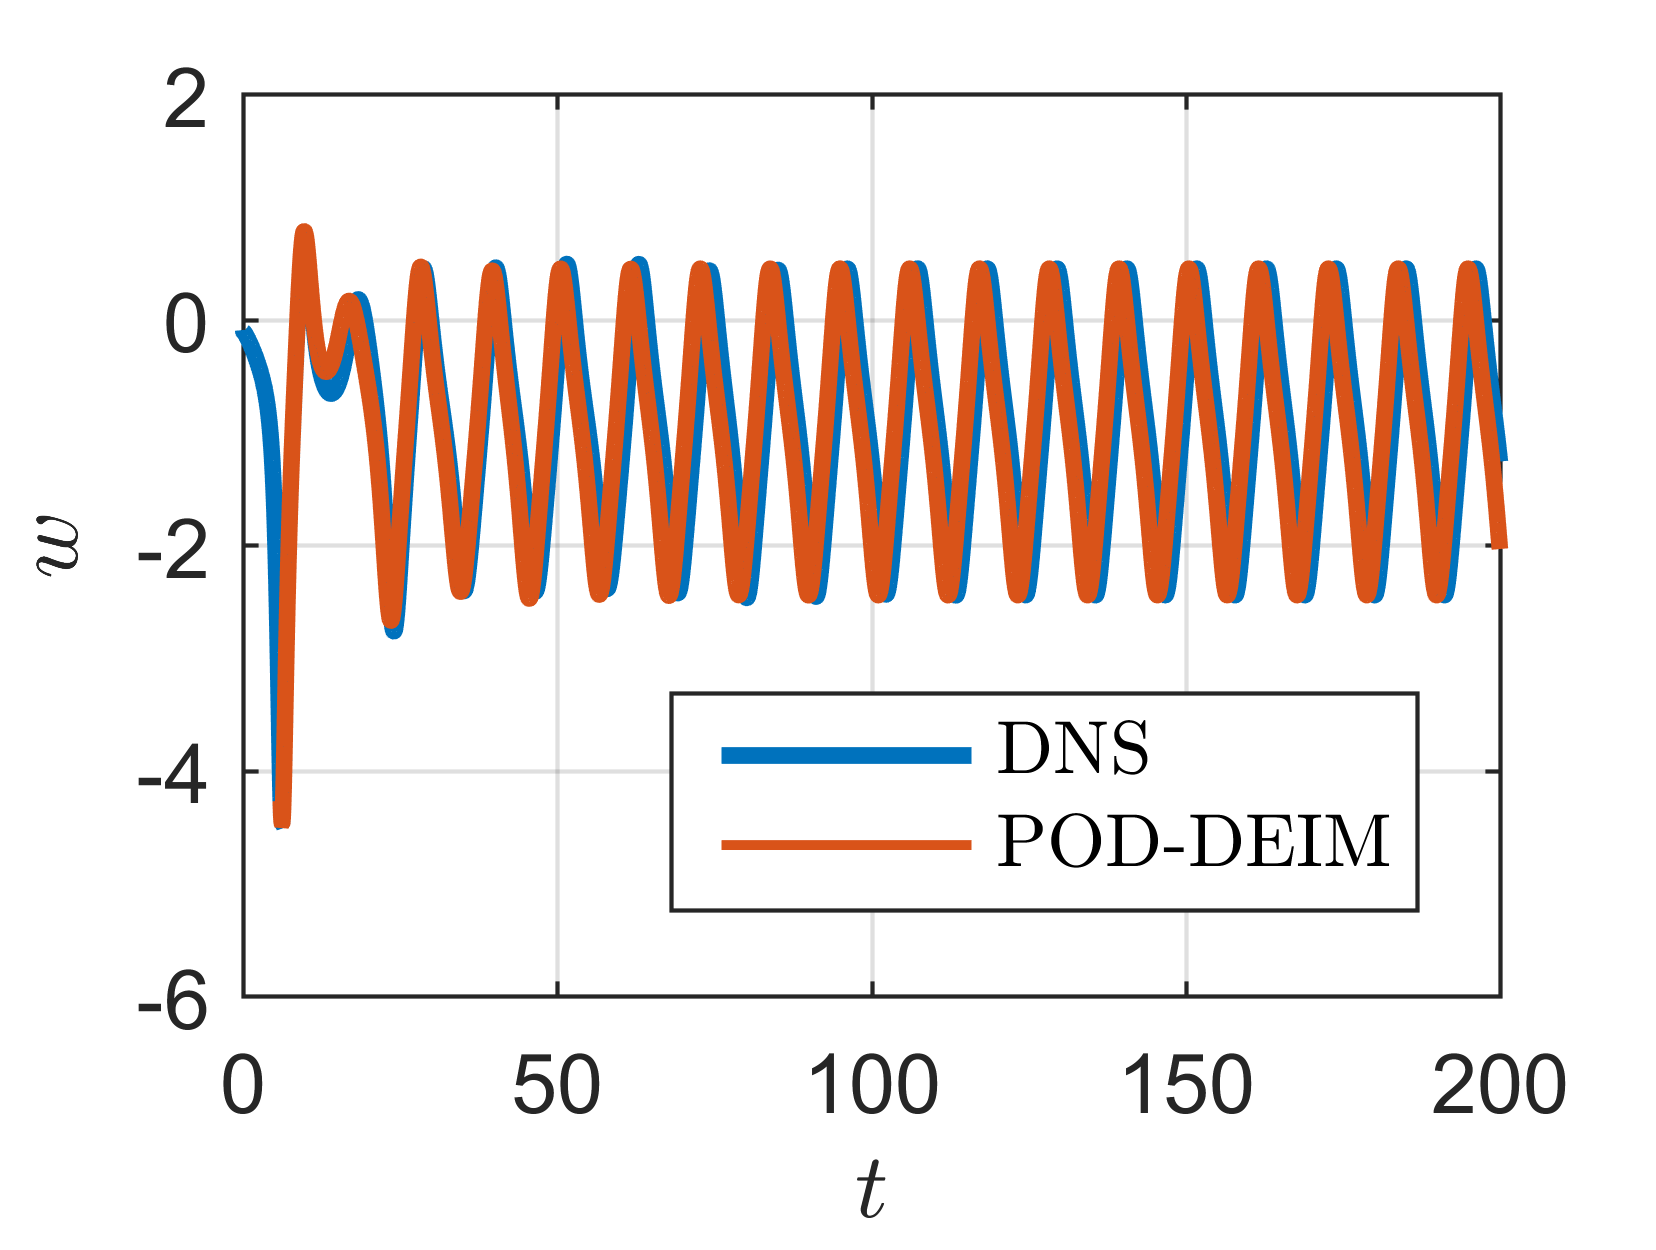
\includegraphics{TimeEvononparallel2}
    \hfill
    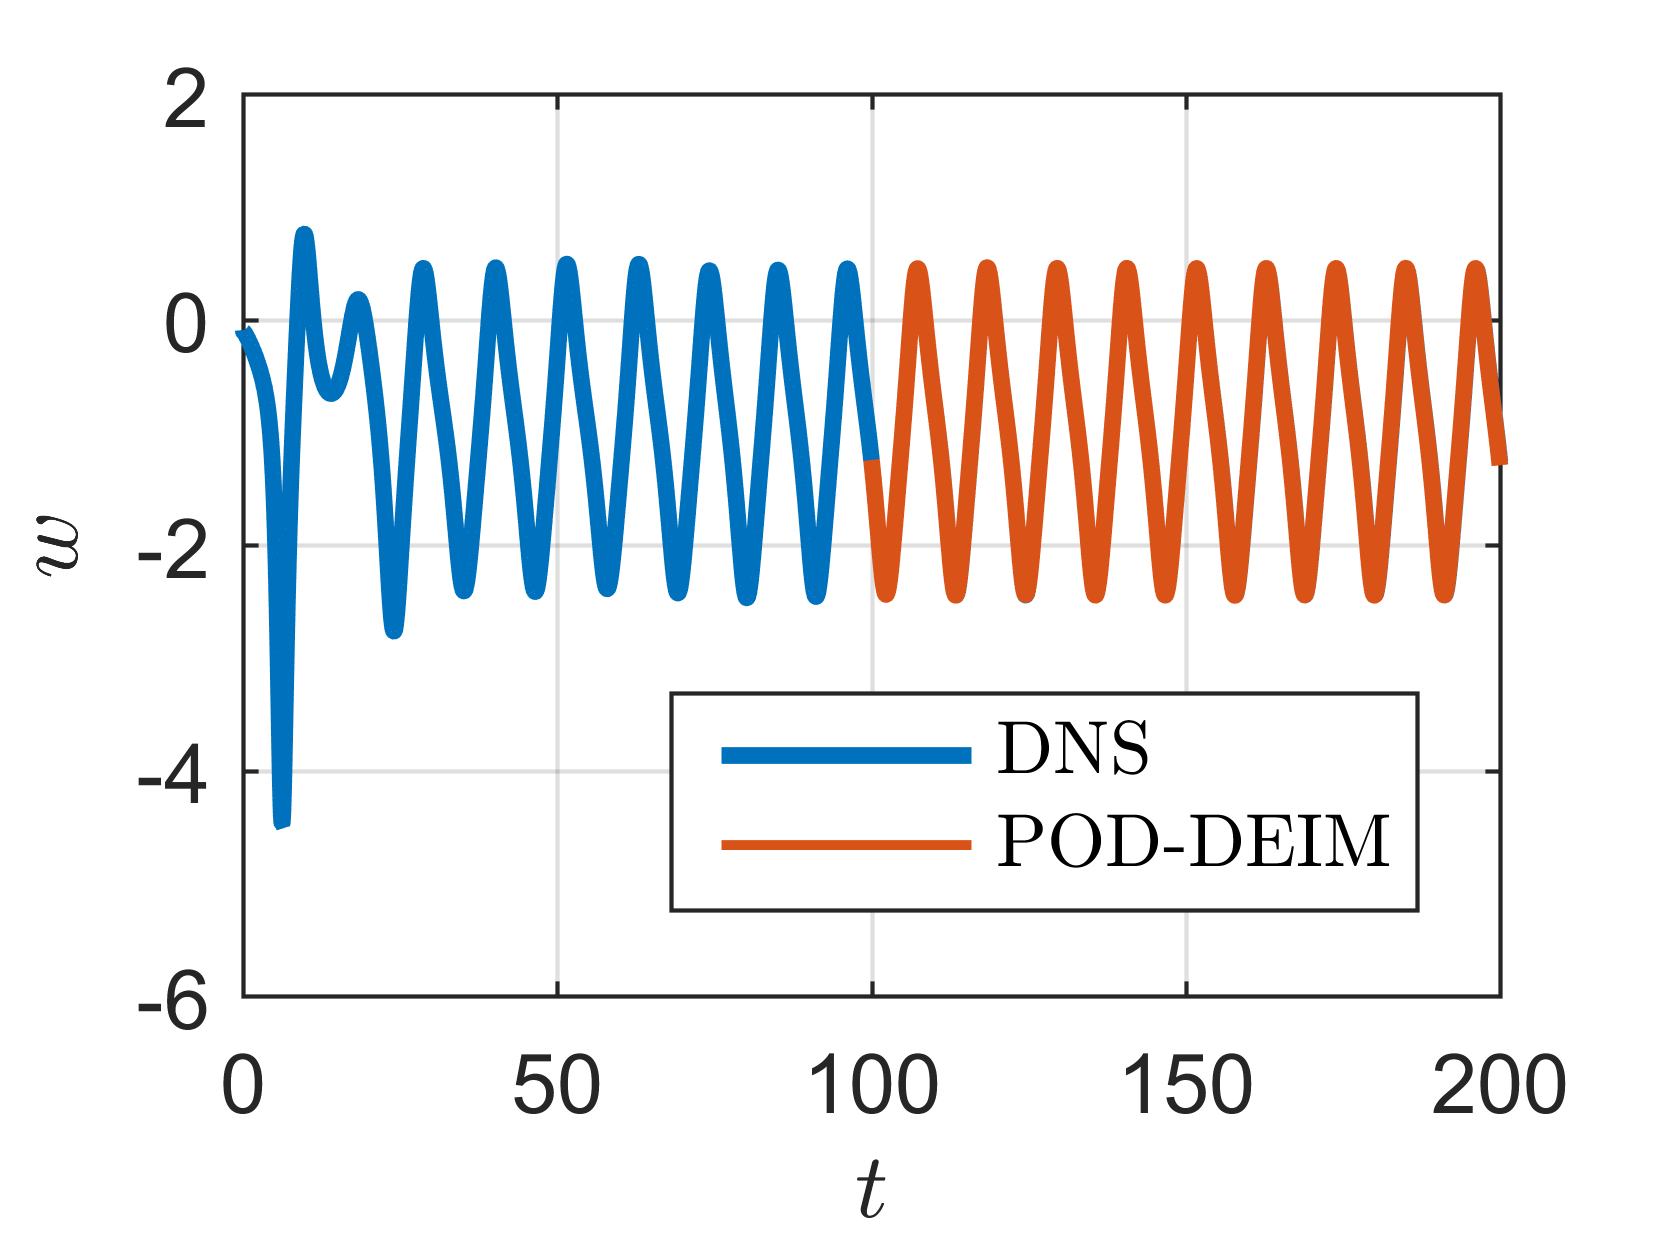
\includegraphics{TimeEvononparallel1}
    \caption{%
    	    (a) limit cycle modes for transient and (b) transient modes for limit cycle.
        }
    \label{fig:TImeEvononparallel}
\end{figure}

The other case of predicting limit cycle from transient modes do not introduce the discrepancy in the initial condition because the last snapshots is used as initial condition for the ROM, Fig \ref{fig:TImeEvononparallel} (b). However we cannot retrieve the same accuracy as for limit cycle modes reproducing limit cycle behaviour. Another choice to obtain all the dynamic of the system is to built the mode on the transient part of the signal including a part of limit cycles. The POD basis will so reproduce faithfully the DNS snapshots in each regime, and the dynamic will be better captured. Table \ref{tab:errorcyclenon} present the error on the limit cycle as the transient modes include progressively the limit cycle snapshots. This technique allows us to increase the accuracy of the ROM when transient and limit cycle behaviour want to be captured.

\begin{table}[!ht]
\begin{center}
\begin{tabular}{ c || c | c | c | c | c |c|}
%\hline
 Transient modes  & $t\in[0.5,70]$ & $t\in[0.5,100]$ & $t\in[0.5,160]$ & $t\in[0.5,180]$\\ \hline
 relative error on CL & $1\cdot 10^{-1}$ & $9\cdot 10^{-3}$ & $2\cdot 10^{-3}$  & $2\cdot 10^{-3}$ \\ \hline
\hline
\end{tabular}
\caption{Relative errors of the ROM for the nonparallel case with respect to the DNS on 10 limit cycles when the ROM start at $t=0.5$\label{tab:errorcyclenon}}
\end{center}
\end{table}

\section{Conclusions}
\label{sec:conclusions}

We have analyzed the parallel and non-parallel {\KSE}s from the perspective of stable solutions and POD-DEIM models.
The eigendecomposition of the linearized parallel dynamics about the trivial base flow reveals that the longest wave mode is the least stable one.
On the other hand, the eigendecomposition of the non-parallel equation is treated numerically.
When the coefficient of the stabilizing fourth derivative is decreased, the stable solution of both equations evolves from the base flow to a simple periodic orbit of a single frequency, and further to a periodic orbit exhibiting multiple harmonics.

In the parallel equation, the state POD modes are simple sinusoids.
The DEIM points are scattered throughout the domain because the periodicity creates spatial invariance.
Considering only the saturated periodic orbit, 8-mode POD-DEIM models capture simple periodic orbits extremely well, and 6-mode models exhibit small errors the time periodicity.
Furthermore, POD-DEIM models computed only from the transient growth, as well as only from the periodic orbit, are both able to capture the entirety of the transient and saturated dynamics.
A greater number of modes may be required for accurate modeling, however, especially when the periodic orbit exhibits multiple frequencies.

\section{Acknowledgements}

We would like to thank ERCOFTAC for funding and providing the 2016 Montestigliano Spring School.
We are also deeply grateful for Denis Sipp, Peter Schmid, and Shervin Bagheri for leading the school.
K. K. C. was supported by the Viterbi Postdoctoral Fellowship through the Viterbi School of Engineering at the University of Southern California.
\kkc{Victor, Emma, Simon---add your funding sources and other acknowledgements here.}

Simon Pasche is supported by the Swiss National Science Foundation.

\bibliography{BeltranChenCookePasche}

\end{document}

%%% Local Variables:
%%% mode: latex
%%% TeX-master: t
%%% End:
